\documentclass[a4paper]{article}
\usepackage{amsmath}
\usepackage{cite}
\usepackage{graphicx}
\usepackage[utf8]{inputenc}
\usepackage[T1]{fontenc}
\usepackage{lmodern}
\usepackage[ngerman]{babel}
\usepackage{hyphenat}
\usepackage{placeins}
\usepackage{subfig}
\usepackage{hyperref}
\usepackage{listings}

\title{Algorithmen und Datenstrukturen Hausarbeit:\\Vergleich von Bäumen}
\author{Hugo Protsch}
\usepackage[a4paper, total={6in, 8in}]{geometry}

\begin{document}

    \maketitle
    \tableofcontents
    \newpage
    \section*{Einleitung}\label{sec:Einleitung}
    \addcontentsline{toc}{section}{Einleitung}

    In der ersten Praktikumsaufgabe haben wir binäre Suchbäume betrachtet.
    Wir haben festgestellt, dass diese im Vergleich zu verketteten Listen eine erheblich
    bessere Laufzeit aufweisen, da beim Traversieren des Baumes nur über die
    Höhe des Baumes gelaufen wird, statt, wie bei der Liste, über jedes Element.

    Es fiel jedoch auf, dass der Vorteil beim Einfügen von aufsteigenden und
    absteigenden Zahlen verloren geht.
    Hierbei entsteht ein Baum, der entartet, also nicht balanciert, ist.
    Im Extremfall entsteht somit eine einfach verkettete Liste.
    Die Laufzeit von Einfüge-, Lösch- und Suchoperationen
    ist in diesem Fall wieder linear (\(O(n)\)).
    Um eine solche Entartung der Bäume und die daraus resultierende verminderte Performance
    zu vermeiden, muss also eine Strategie entwickeln werden, die den Baum balanciert hält.
    Ein Ansatz, der in Abschnitt~\ref{sec:avl-tree} betrachtet wird, ist der AVL-Baum,
    der jeweils beim Einfügen und Löschen von Elementen die
    Balance des Baumes überprüft und im Falle der Entartung diese sofort ausgleicht.

    Eine zweite Variation des binären Suchbaumes, die in Abschnitt~\ref{sec:splay-tree}
    betrachtet wird, ist der Splay-Tree.
    Dieser hat das Ziel, Elemente, die häufig zugegriffen werden, im Baum möglichst weit oben zu
    halten und somit die Zugriffszeit auf diese zu verringern.
    Anders als beim AVL-Baum, wird ein Splay-Tree nicht balanciert, somit kann der Baum, wie ein
    normaler Binärbaum, entarten.
    Der Vorteil liegt also lediglich beim wiederholten Zugriff auf eine kleine Teilmenge der im
    Baum befindlichen Elementen.

    In beiden Abschnitten werden doppelte Schlüsselwerte in den Bäumen nicht
    erlaubt.


    \section{AVL Tree}\label{sec:avl-tree}
    \subsection{Algorithmus}\label{subsec:algorithmus}

\subsubsection{AVL-Bedingung}
Ein AVL-Baum ist ein Binärbaum, der die zusätzliche Eigenschaft besitzt, dass
die Balance, die als die Differenz der Höhe $h$ der beiden
Teilbäume definiert ist (siehe Formel~\ref{eq:balance}), bei jedem Knoten mindestens 1 und
maximal 1 beträgt.
Diese Eigenschaft wird AVL-Bedingung genannt.
Dabei ist die Höhe analog zum regulären Binärbaum definiert (siehe Formel~\ref{eq:height}).

\begin{equation}
    bal(k) = h(T_r) - h(T_l)\label{eq:balance} \in \{-1,0,1\}
\end{equation}
\begin{equation}
    h(k) = max(h(T_l), h(T_r))\label{eq:height}
\end{equation}
Durch diese Bedingung wird sichergestellt, dass der Baum zu jedem Zeitpunkt
balanciert ist und somit das in der Einleitung beschriebene Problem der
schlechten Laufzeit des Binärbaumes durch Entartung nicht auftreten kann.

\subsubsection{Rebalancierung}\label{par:rebalancing}
Nach dem Einfügen und Löschen von Elementen kann es jeweils vorkommen, dass die
Balance eines Konten -2 oder 2 beträgt.
Somit muss der AVL-Baum nach diesen Operationen die AVL-Bedingung überprüfen,
und eventuell eine Rebalancierung vornehmen.
Dabei wird zwischen insgesamt vier Fällen unterschieden, die durch die Folge
der Balancewerte definiert sind (siehe auch Abbildung~\ref{fig:AVL-Cases}):
\begin{enumerate}
    \item Left Left: -2/-1 oder -2/0 → Rechtsrotation\label{enm:rebal1}
    \item Right Right: +2/+1 oder +2/0 → Linksrotation \label{enm:rebal2}
    \item Left Right: -2/+1 → Doppelte Rechtsrotation \label{enm:rebal3}
    \item Right Left: +2/-1 → Doppelte Linksrotation \label{enm:rebal4}
\end{enumerate}
Die ersten beiden und letzten beiden Fälle sind dabei jeweils symmetrisch zueinander.

\paragraph*{Rotation}\label{par:rotating}

Die Rebalancierung wird mithilfe von Rotationen von Knoten vorgenommen.
Bei einer Rotation wird immer ein Knoten als Wurzelknoten betrachtet.
Alle Knoten, die über dem Wurzelknoten stehen, sind für die Rotation nicht von
Relevanz.
%Im Left Left bzw. Right Right Case ist dies der Knoten,
%bei dem die AVL-Bedingung verletzt wird.
Der Wurzelknoten wird mit dem Kindknoten rotiert, auf dessen Seite die
Unbalance vorliegt, im Folgenden wird dieses Kind Rotationsknoten genannt:
\begin{itemize}
    \item Linksrotation: Rotieren vom Wurzelknoten mit rechtem Kindknoten
    \item Rechtsrotation: Rotieren vom Wurzelknoten mit linken Kindknoten
\end{itemize}
Betrachte Abbildung~\ref{fig:AVL-Cases}~(Left~Left~Case).
Zum Rotieren der beiden Knoten nach rechts werden folgende Operationen ausgeführt:
\begin{enumerate}
    \item Der Wurzelknoten (5) wird als rechtes Kind vom Rotationsknoten (4)
    gesetzt\label{enm:reblStep1}
    \item Der eben ersetzte Knoten (C) (rechtes Kind vom Rotationsknoten) wird als linkes Kind
    des ursprünglichen Wurzelknotens (5) gesetzt\label{enm:reblStep2}
    \item Der Rotationsknoten (4) wird als neue Wurzel gesetzt\label{enm:reblStep3}
\end{enumerate}
Dabei muss die Höhe des Rotations- und Wurzelknotens angepasst werden.
Dies lässt sich am leichtesten durch eine erneute Berechnung mit Formel~\ref{eq:height} erzielen.
Des Weiteren muss eventuell die Höhe der Knoten über dem Wurzelknoten angepasst werden.

An Abbildung~\ref{fig:AVL-Cases}~(Balanced) wird deutlich, dass durch die
Rechtsrotation beim Left Left Case die AVL-Bedingung wieder erfüllt ist.

Eine Linksrotation erfolgt symmetrisch.

\subsubsection{Doppelrotation}

Bei den Fällen Left Left und Right Right konnte der Baum mit lediglich
einer Rotation balanciert werden.
Dies reicht bei den anderen Fällen nicht aus, wie wird aus Abbildung~\ref{fig:AVL-wrong-rotate}
ersichtlich wird.

Es müssen insgesamt zwei Rotationen durchgeführt werden:
Mit der ersten Rotation wird der Left Left bzw. Right Right Case
herbeigeführt, die zweite Rotation befriedigt anschließen die AVL-Bedingung.
Betrachte Abbildung~\ref{fig:AVL-Cases} (Left Right Case).
Im Left Right Case wird zunächst eine Linksrotation zwischen dem linken
Kindknoten des Wurzelelementes und des rechten Nachfolgers ausgeführt.
Diese Rotation wird symmetrisch zur oben beschriebenen Rechtsrotation ausgeführt.
Anschließend liegt der Left Left Case vor, eine einfache Rechtsrotation
befriedigt nun die AVL-Bedingung.


\begin{figure}[hbt]
    \centering
    %https://fr.m.wikipedia.org/wiki/Fichier:AVL_Tree_Rebalancing.svg
    %https://github.com/LambdaSchool/Data-Structures
    %https://commons.wikimedia.org/wiki/File:AVL_Tree_Rebalancing_he.svg
    \begin{minipage}[c]{.45\textwidth}
        \subfloat[Korrekt]{
            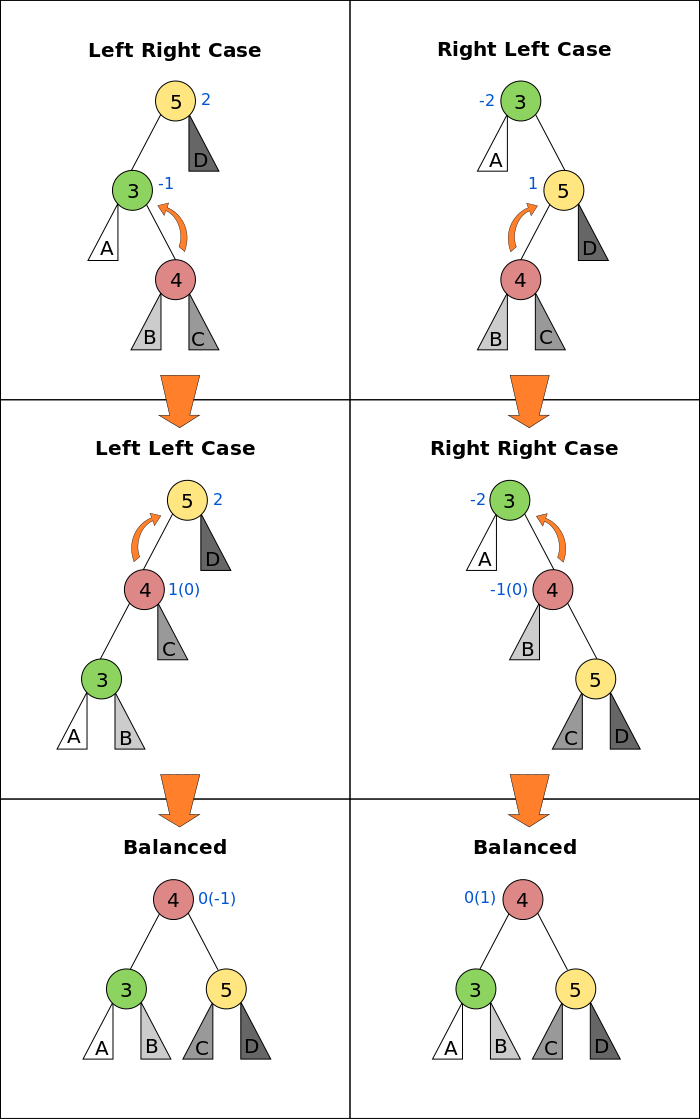
\includegraphics[width=.95\linewidth]{img/external/AVL_Tree_Rebalancing}
            \label{fig:AVL-Cases}}
    \end{minipage}
    \begin{minipage}[c]{.45\textwidth}
        \subfloat[Falsch]{
            \includegraphics[width=.95\linewidth]{img/external/AVL_Tree_Rebalancing_wrong.pdf}
            \label{fig:AVL-wrong-rotate}}
    \end{minipage}
    \caption{Rebalancierung}
    \label{fig:rebalancing}
\end{figure}
%\begin{figure}[hbt]
%    \centering
%    \includegraphics[width= 0.45\textwidth]{img/AVL_Tree_Rebalancing_wrong.pdf}
%    \caption{Falsche Rotation}
%\end{figure}

\subsection{Entwurf}\label{subsec:entwurf2}

\subsubsection{InitBT, IsEmptyBT, EqualBT, FindBT}
Die Implementation dieser Methoden kann aus der Implementation des Binärbaumes übernommen werden.
Bei der InitBT Methode müssen lediglich alle Counter der Rotationszählung zurückgesetzt werden.

\subsubsection{IsBT}\label{par:avl-isBT}
Die Methode von dem Binärbaum wird um die Überprüfung der AVL-Bedingung erweitert.
Dabei wird bei jedem Knoten zusätzlich überprüft, ob die Balance (siehe Formel~\ref{eq:balance})
-1, 0 oder +1 beträgt.
Der Ausdruck wird mit den bisherigen Ausdrücken und-verknüpft.

\subsubsection{InsertBT, DeleteBT}
Das Einfügen und Löschen wird wie bei einem Binärbaum realisiert.
Die einzige Änderung, die vorgenommen werden muss, ist das Prüfen der
AVL-Bedingung und eventuelles Rotieren, bottom-up nach dem Einfügen bzw. Löschen.
Dies wird mithilfe der \verb|Rebalance|-Methode vorgenommen, die in
Abschnitt~\ref{par:MethodRebalance} weiter ausgeführt wird.
Beim Löschen muss darauf geachtet werden, dass der Pfad vom tatsächlich entfernten Knoten, also
dem Substitution-Knoten, überprüft wird.
In Abbildung~\ref{fig:AVL-insert} und~\ref{fig:AVL-delete} sind die notwendigen Änderungen jeweils
blau markiert.

\begin{figure}[htbp]
    \centering
    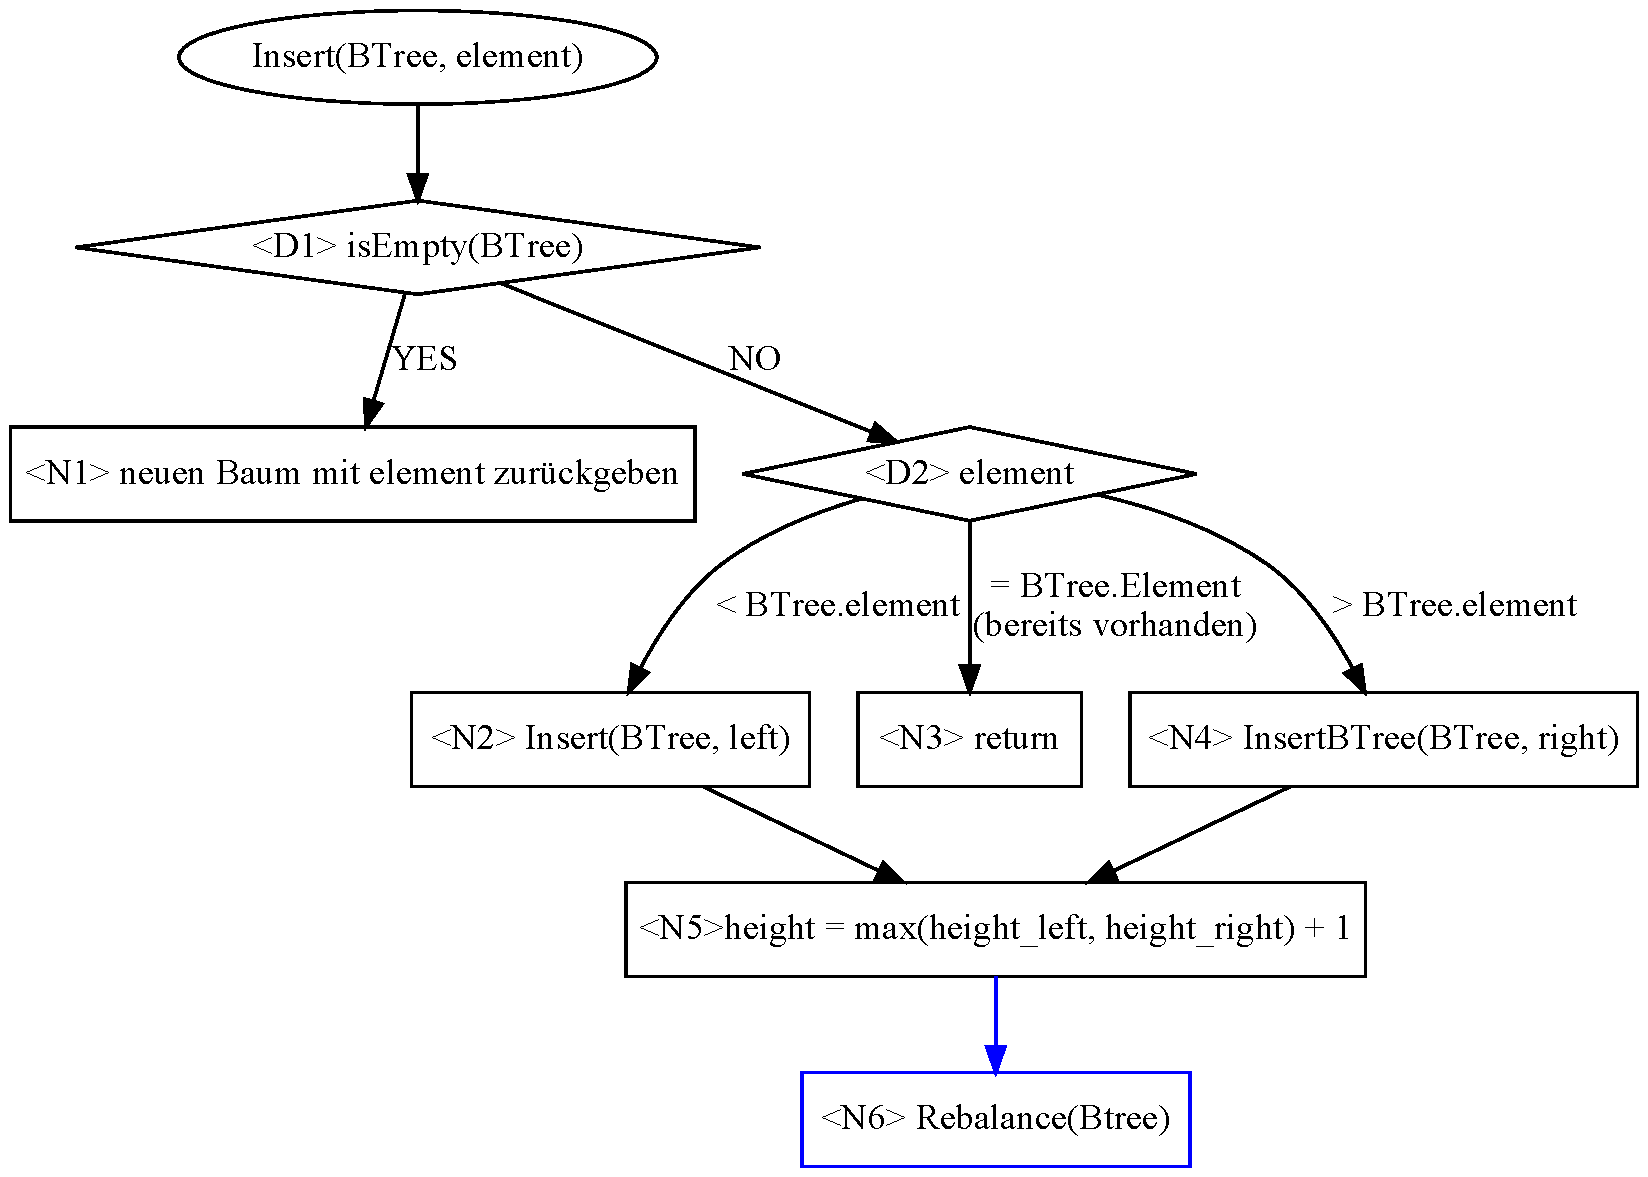
\includegraphics[width= 0.70\textwidth]{img/gv/insert}
    \caption{InsertBT}
    \label{fig:AVL-insert}
\end{figure}
\begin{figure}[p]
    \centering
    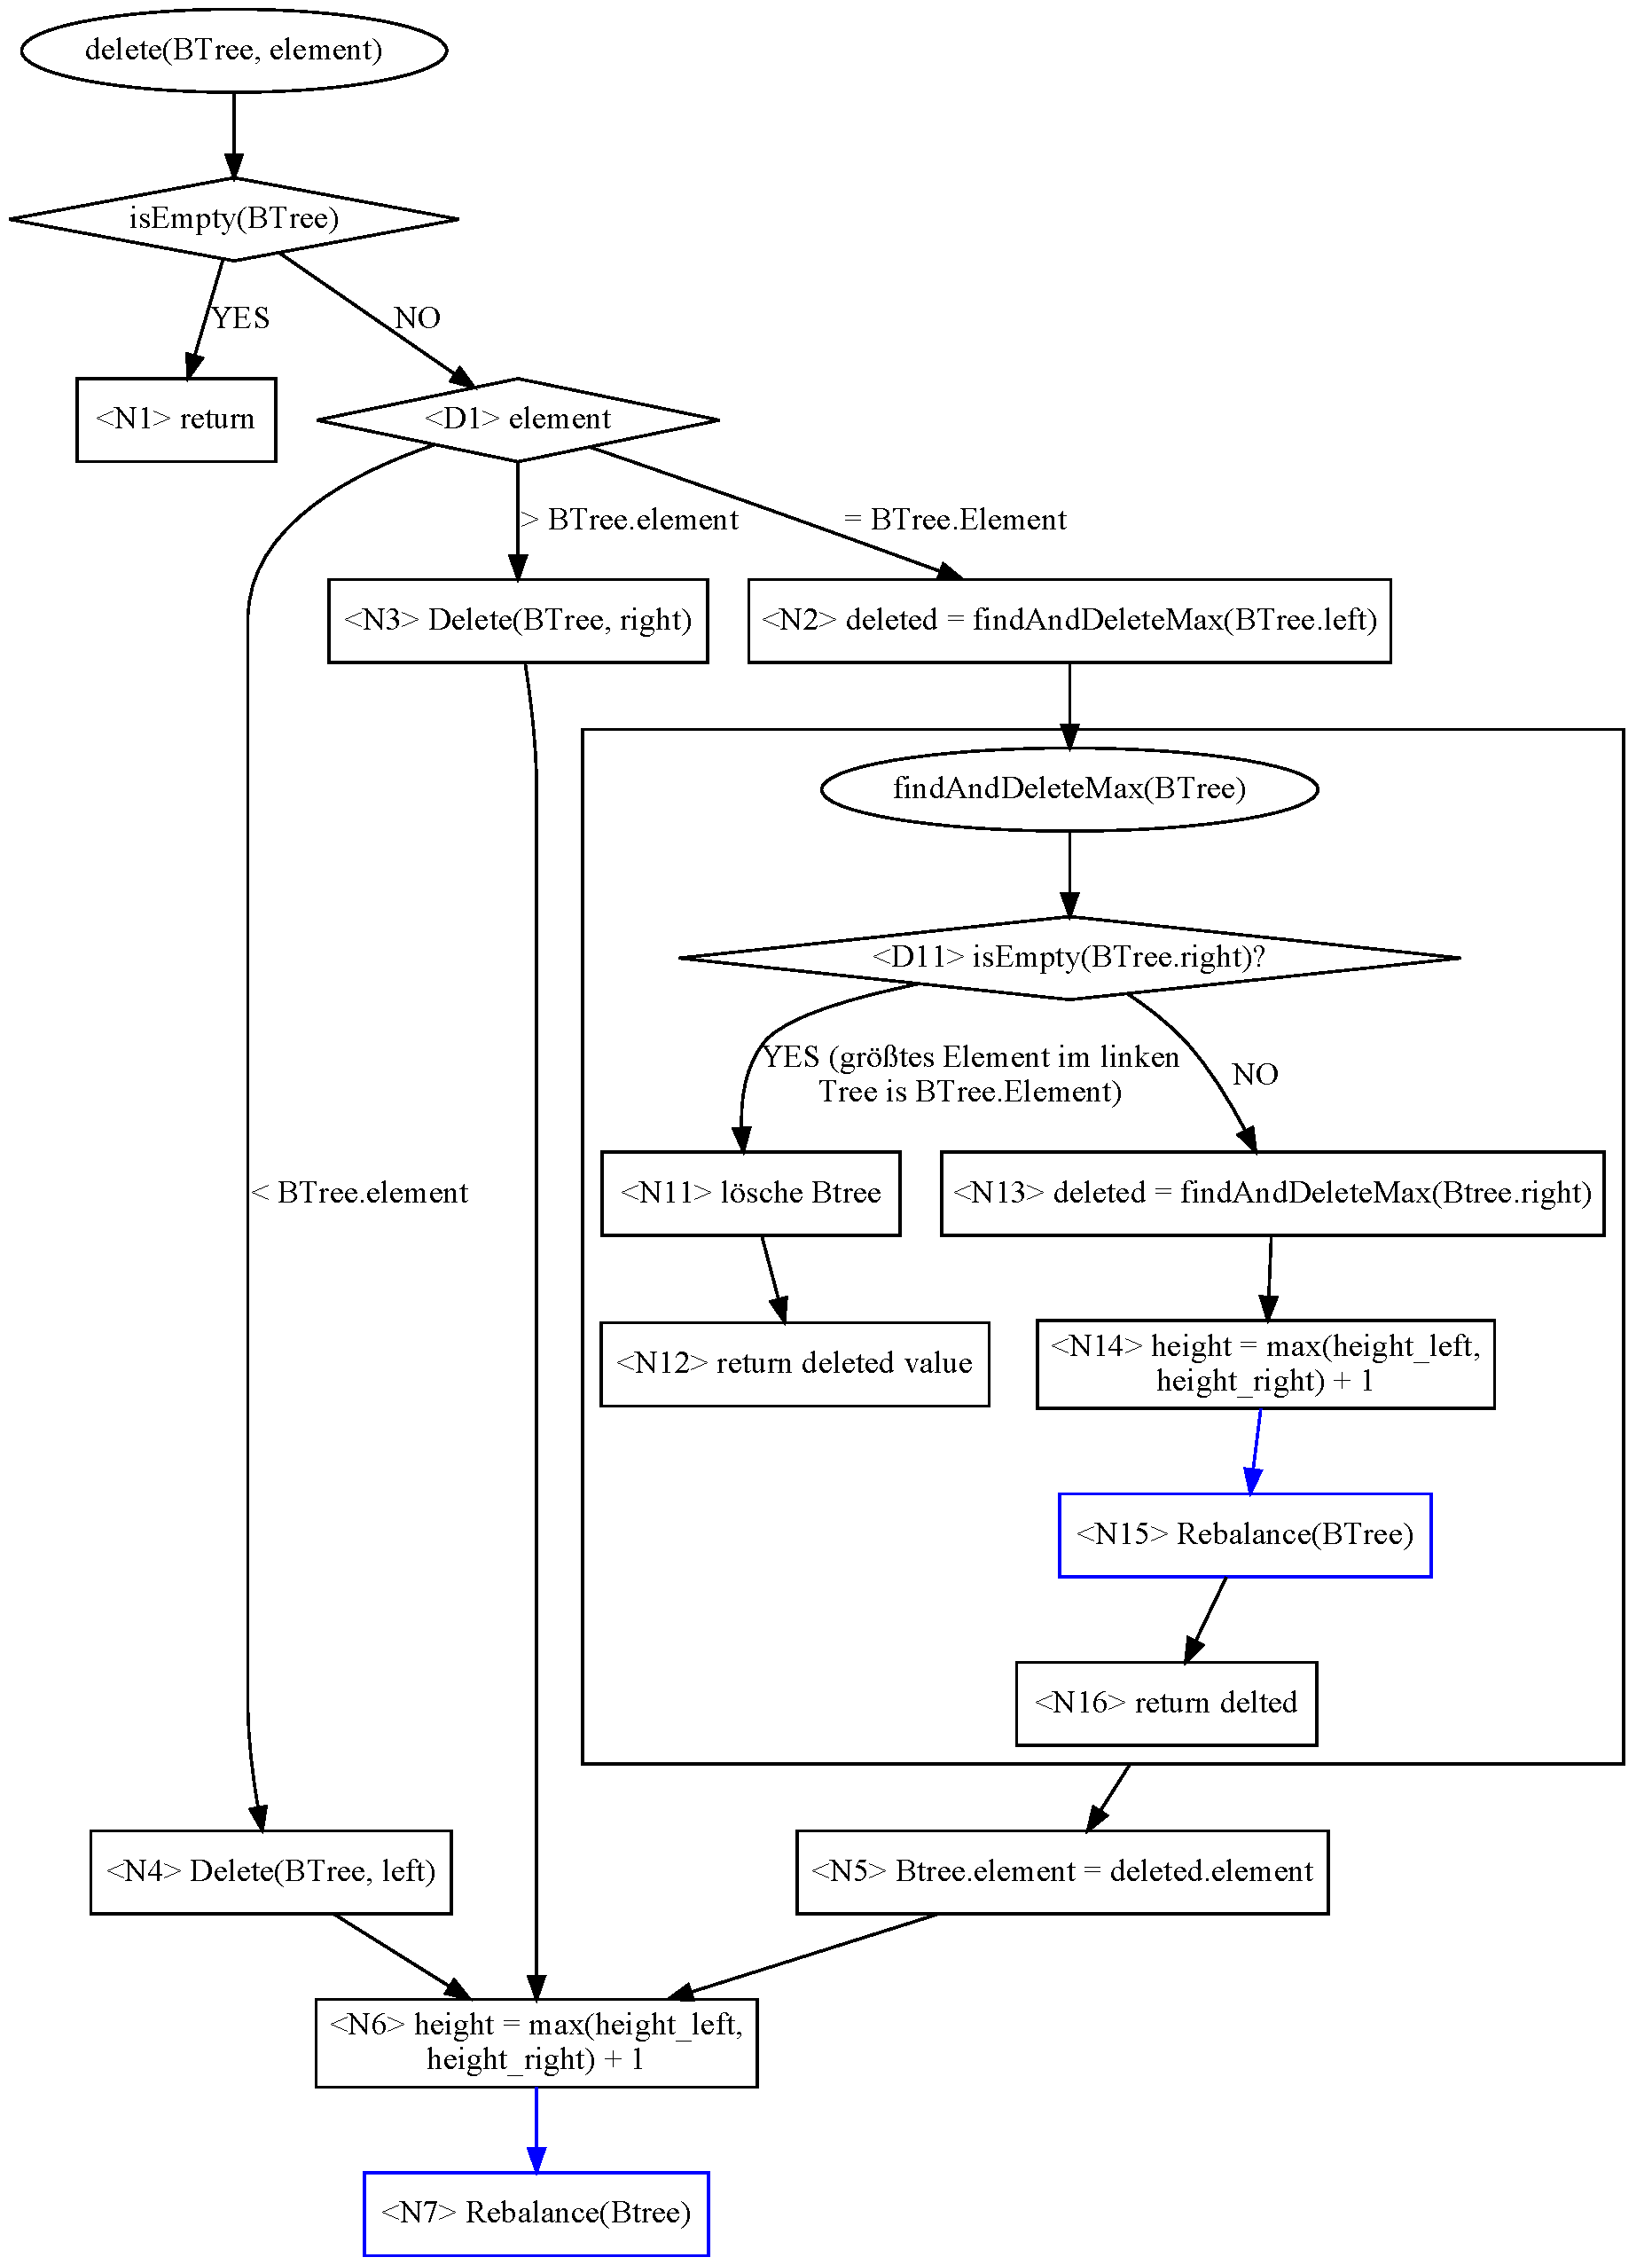
\includegraphics[height= 0.97\textheight]{img/gv/delete}
    \caption{DeleteBT}
    \label{fig:AVL-delete}
\end{figure}

\subsubsection{PrintBT}\label{par:printBT}
Diese Funktion speichert eine Representation des übergebenen Baumes als Datei im GraphViz Format.
Dafür wird am Anfang einmal der Header (\verb|digraph G{|), dann der Inhalt, am Ende eine
schließende Klammer ausgegeben.
Um den Inhalt auszugeben werden für jeden Knoten bis zu drei Zeilen ausgegeben:
\begin{enumerate}
    \item \verb|<Knoten> -> <Linkes Kind>;|
    \item \verb|<Knoten> -> <Rechtes Kind>;|
    \item \verb|<Knoten> [label = "<Knoten>\n(<Hoehe von Knoten>)" color = <Farbe>];|
\end{enumerate}
Dabei entspricht \verb|Knoten, Linkes Kind, Rechtes Kind| dem Wert des jeweiligen Knotens.
Falls ein Kindknoten leer sein sollte, wird dafür nur die letzte Zeile ausgegeben.
Diese formatiert den Knoten selber, dabei wird die Farbe abhängig der Balance gesetzt.

Knoten mit der Balance von \(-1\) werden violett, mit der Balance von \(+1\)
blau, mit der Balance von \(0\) schwarz dargestellt.
Falls die AVL-Bedingung nicht eingehalten wird, erscheint der Knoten rot.

\subsubsection{Rebalance}\label{par:MethodRebalance}
Die \verb|Rebalance|-Methode bekommt einen Knoten übergeben, überprüft die AVL-Bedingung und
balanciert den Knoten durch Rotieren, falls die AVL-Bedingung nicht erfüllt ist.
Dafür wird zunächst die Balance des übergebenen Knotens überprüft.
Falls diese -1, 0, +1 beträgt, wird der Knoten nicht verändert.
Andernfalls wird überprüft, welcher der in Abschnitt \ref{par:rebalancing} aufgeführten Fälle
vorliegt und die nötigen Rotationen mithilfe der~\nameref{par:MethodRotate}-Methode ausgeführt.
Falls eine Doppelrotation ausgeführt wird, wird außerdem der entsprechende Counter erhöht.
In Abbildung~\ref{fig:rebalance} wird die Methode in einem Flussdiagramm dargestellt.
\begin{figure}[p]
    \centering
    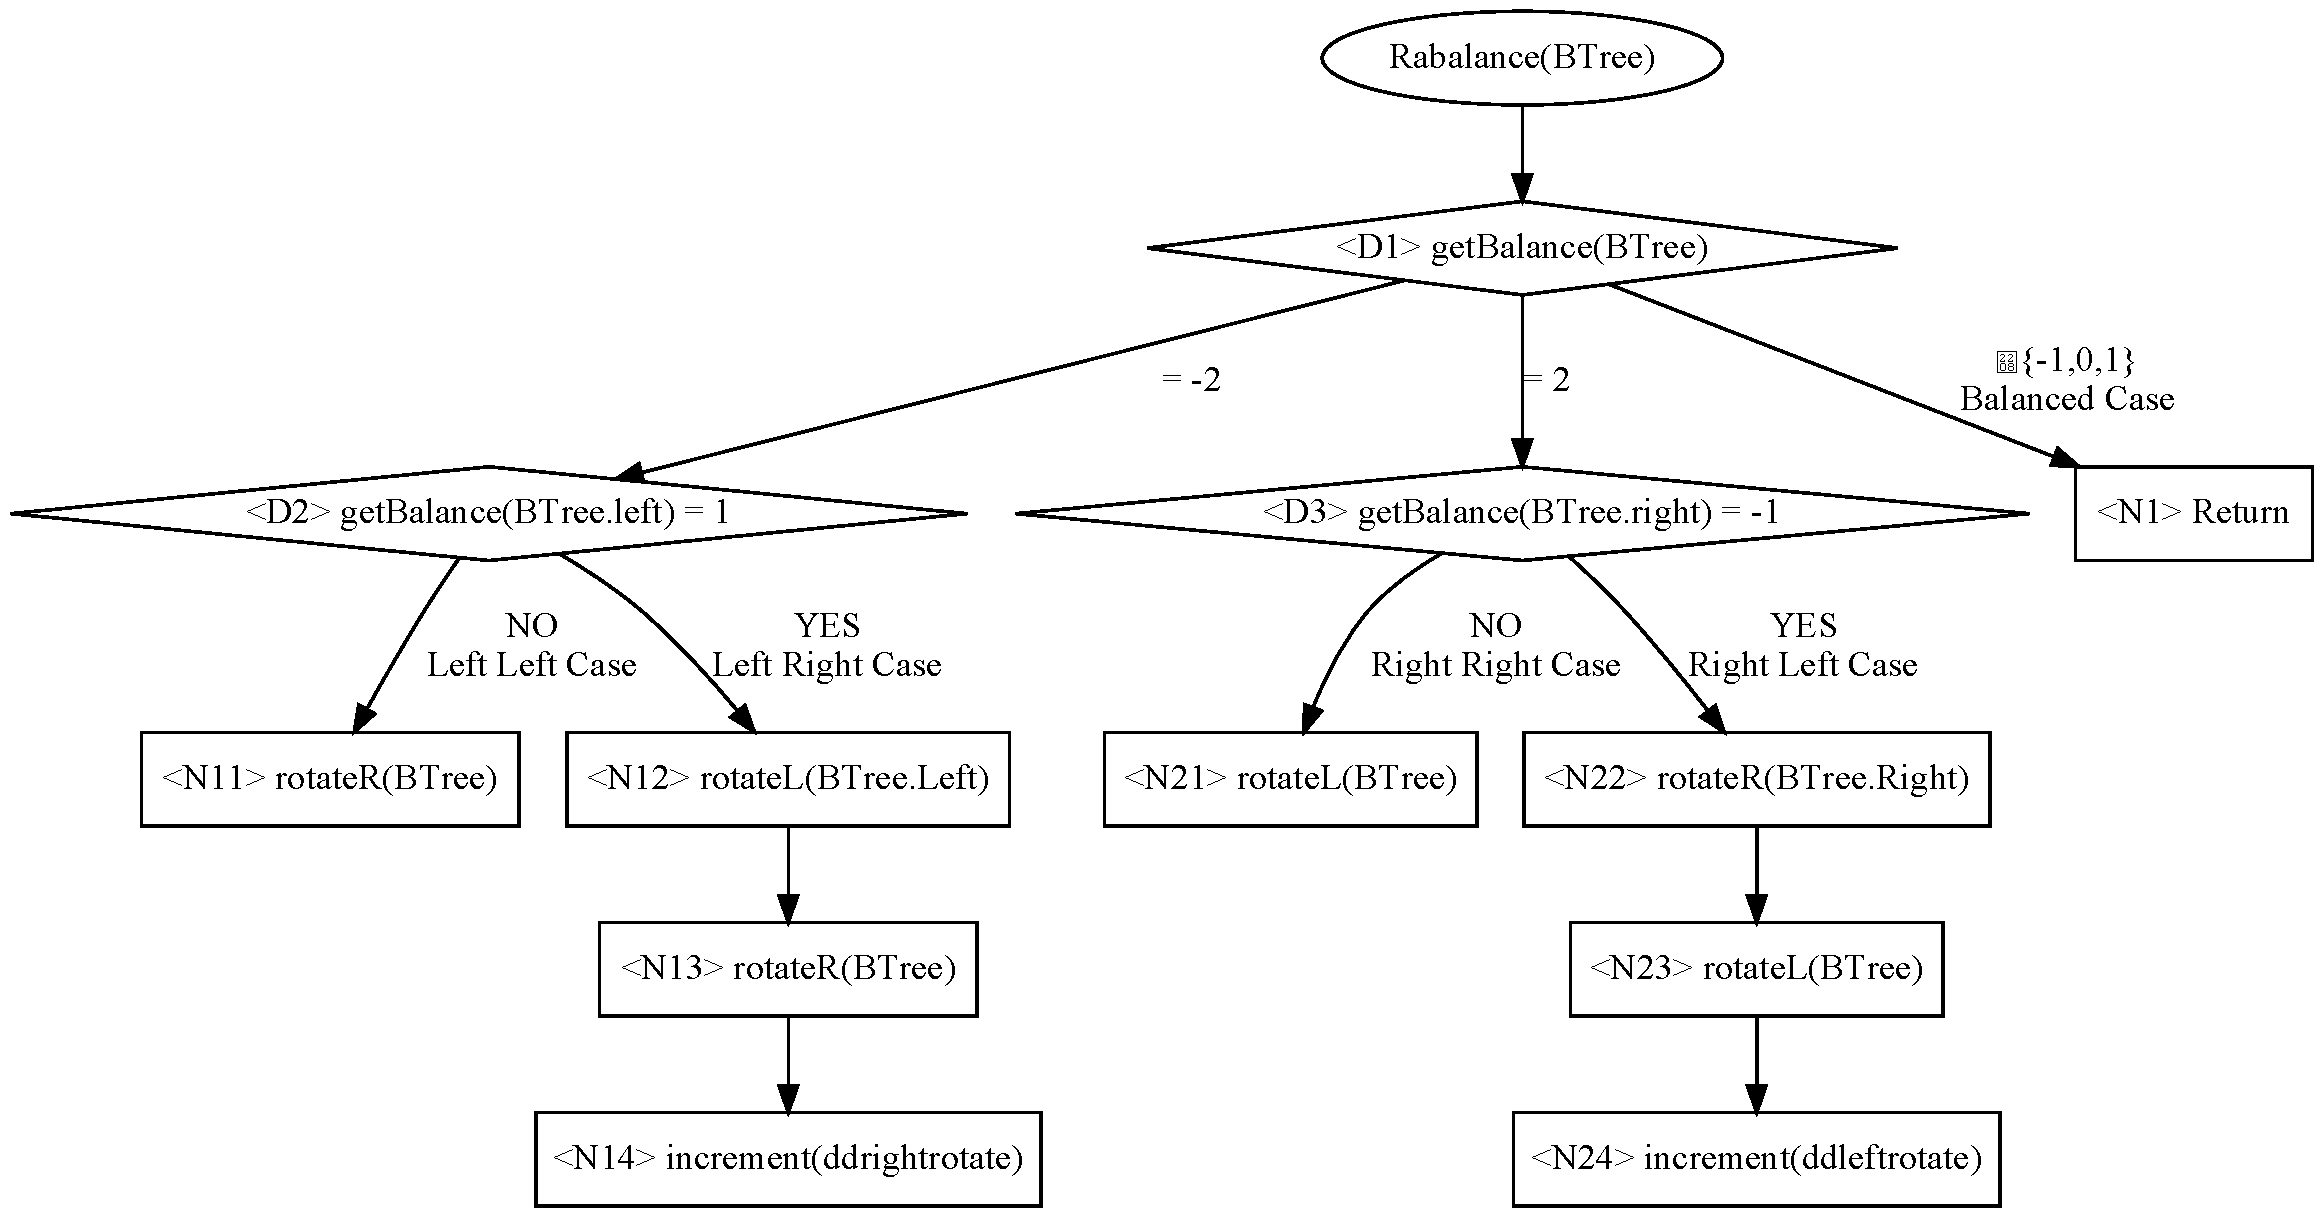
\includegraphics[width = 0.85\textwidth]{img/gv/rebalance}
    \caption{Rebalancierung}
    \label{fig:rebalance}
\end{figure}

\subsubsection{Rotate}\label{par:MethodRotate}
Das Rotieren wurde in Abschnitt~\ref{par:rotating} dargestellt.
In Abbildung~\ref{fig:rotate} wird die Rechts- und Linksrotation zusätzlich in jeweils einem
Flussdiagramm dargestellt.
\begin{figure}[hbtp]
    \centering
    \subfloat[\centering Links]{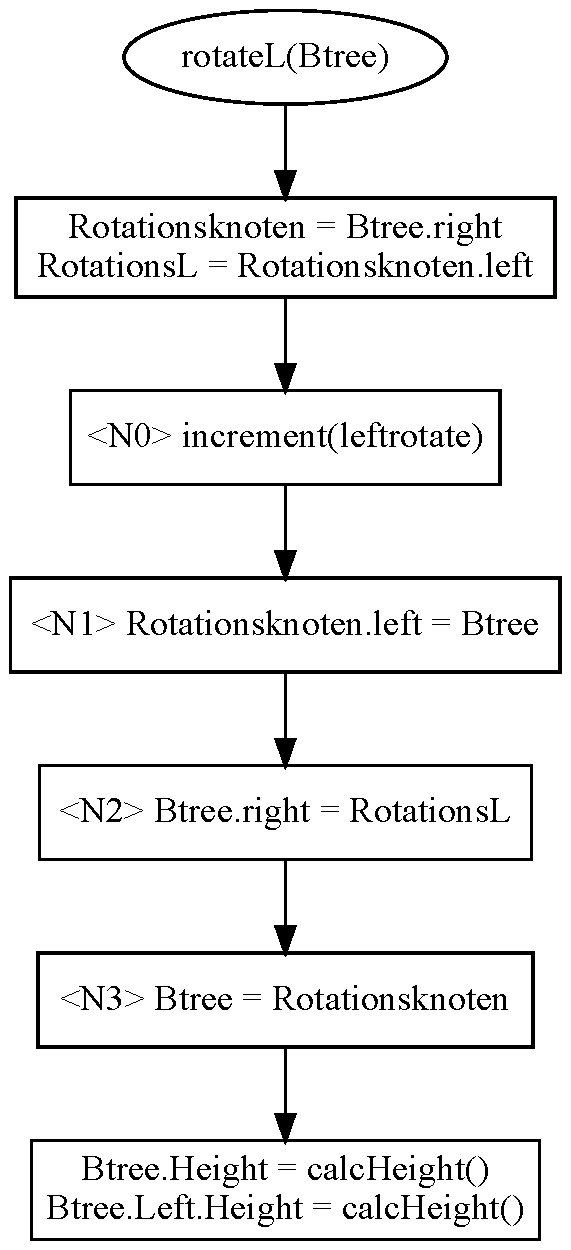
\includegraphics[width = 0.25\textwidth]{img/gv/rotateL.pdf}}
    \subfloat[\centering Rechts]{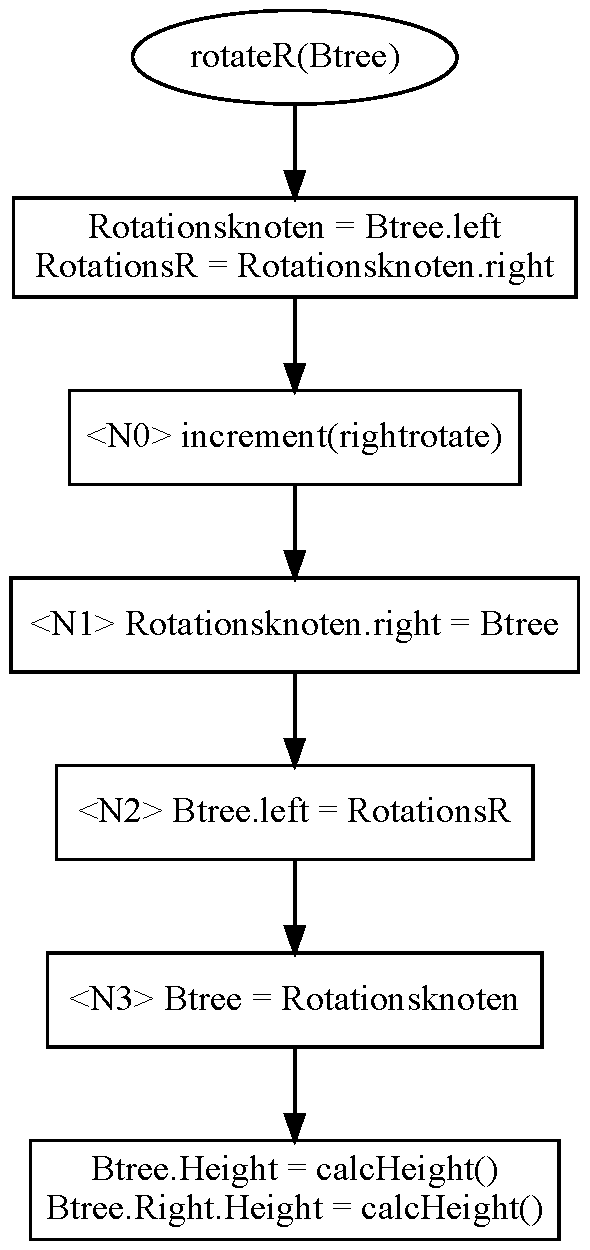
\includegraphics[width = 0.25\textwidth]{img/gv/rotateR.pdf}}
    \caption{Rotieren}
    \label{fig:rotate}
\end{figure}

\FloatBarrier

\subsection{Aufgaben}\label{subsec:aufgaben}

\subsubsection{Aufgabe 1.4 - Analysieren beispielhafter Bäume}
Beispielhafte Bäume werden mit der zur verfügung gestellten Methode\\
\verb|analyseBT:test(<Anzahl Elemente>)| analysiert.

\subparagraph{100 Elemente}
Ein Aufruf mit 100 Elementen ergibt folgende Ausgabe:
\begin{verbatim}
>analyseBT:test(100).
Bei gegebener Höhe 8:
         minimale Anzahl Knoten: 54.
         maximale Anzahl Knoten: 255
Bei gegebener Anzahl an Knoten 100:
         minimale Höhe: 6.
         maximale Höhe: 9
Durchschnittliche Balancefehler: 0.28
         maximaler Balancefehler: 1.
\end{verbatim}

An der Ausgabe ist zu erkennen, dass der erzeugte Baum mit 100 Elementen eine Höhe von 8
aufweist.
Dies liegt innerhalb des theoretischen Rahmens für AVL Bäume der Elementanzahl 100 von mindestens
6 und maximal 9.
Die Ausgabe zeigt außerdem die minimale und maximale Elementanzahl für einen Baum der
vorgegebenen Höhe an, die hier bei 54 und 255 liegt.
Der maximale Balancefehler beträgt 1, somit wurde die AVL-Bedingung bei jedem Knoten eingehalten.
Der durchschnittliche Balancefehler beträgt 0.28, somit hatten 28 der 100 Knoten eine Balance
von -1 oder 1.

\subparagraph{1000 Elemente}
Ein Aufruf mit 1000 ergibt folgende Ausgabe:
\begin{verbatim}
>analyseBT:test(1000).
Bei gegebener Höhe 12:
         minimale Anzahl Knoten: 376.
         maximale Anzahl Knoten: 4095
Bei gegebener Anzahl an Knoten 1000:
         minimale Höhe: 9.
         maximale Höhe: 14
Durchschnittliche Balancefehler: 0.321
         maximaler Balancefehler: 1.
\end{verbatim}

Aus der Ausgabe wird ersichtlich, dass die AVL-Bedingung auch bei 1000 Elementen eingehalten wird.
Des Weiteren wird die Logarithmische Natur des AVL-Baumes ersichtlich:
Bei einer Verzehnfachung der Elementanzahl hat sich die Höhe lediglich um dem Faktor 0.5 erhöht.

\subparagraph{Fehlerhafter Baum}
Ein Aufruf mit einem Baum, der an einem Knoten eine Balance von 2 besitzt, ergibt folgende Ausgabe:
\begin{verbatim}
>analyseBT:analyseBT({3, 3, {}, {4, 2, {}, {5, 1, {}, {}}}}).
Bei gegebener Höhe 3:
         minimale Anzahl Knoten: 4.
         maximale Anzahl Knoten: 7
Bei gegebener Anzahl an Knoten 3:
         minimale Höhe: 2.
         maximale Höhe: 1
Durchschnittliche Balancefehler: 1.0
         maximaler Balancefehler: 2.
\end{verbatim}
Der maximale Balancefehler beträgt wie erwartet 2, außerdem liegt die Höhe des Baumes über dem
theoretischen Maximum.
Der Baum ist somit kein AVL-Baum.

\subsubsection{Aufgabe 1.5 - Löschen von 88 Prozent der Zahlen}
Es wird ein Baum aus 100 Zufallszahlen erstellt, anschließen werden zufällig 88 davon wieder
gelöscht.
In Abbildung~\ref{fig:88before} ist der Baum vor dem Löschen zu sehen.
In Abbildung~\ref{fig:88after} ist der Baum nach dem Löschen zu sehen.

\begin{figure}[hbtp]
    \centerline{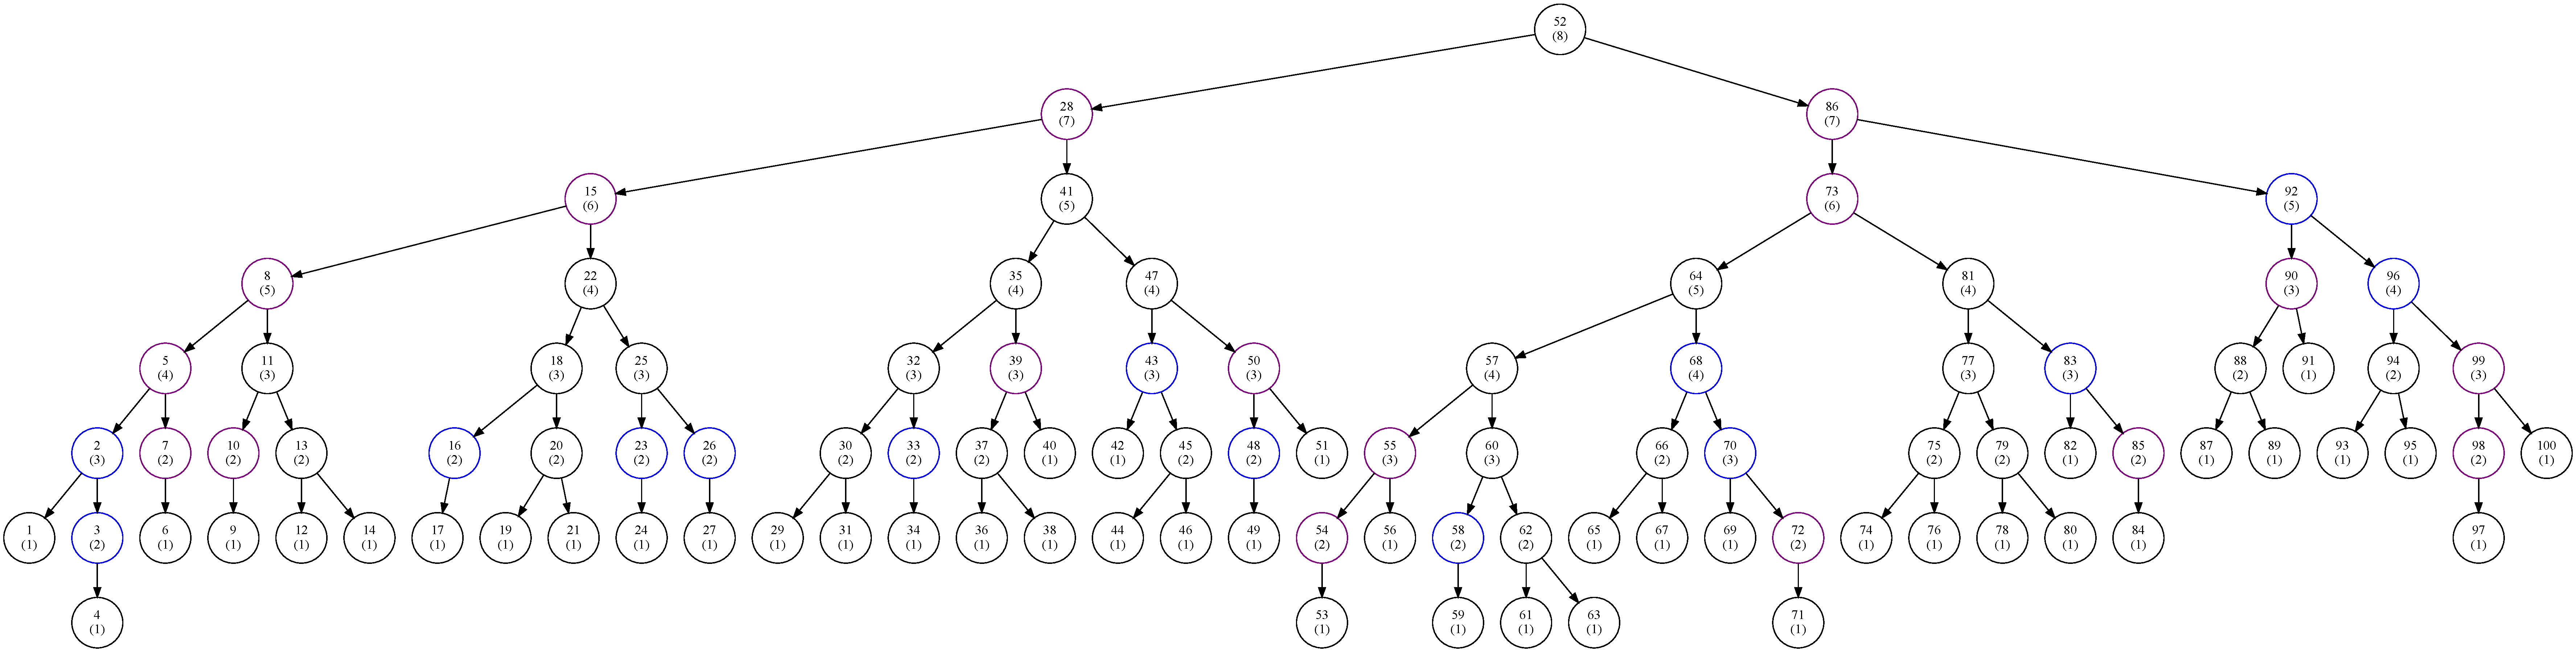
\includegraphics[width = 1.2\textwidth]{img/gv/aufgabe1_6_before.pdf}}
    \caption{Vor dem Löschen}
    \label{fig:88before}
\end{figure}

\begin{figure}[hbtp]
    \centering
    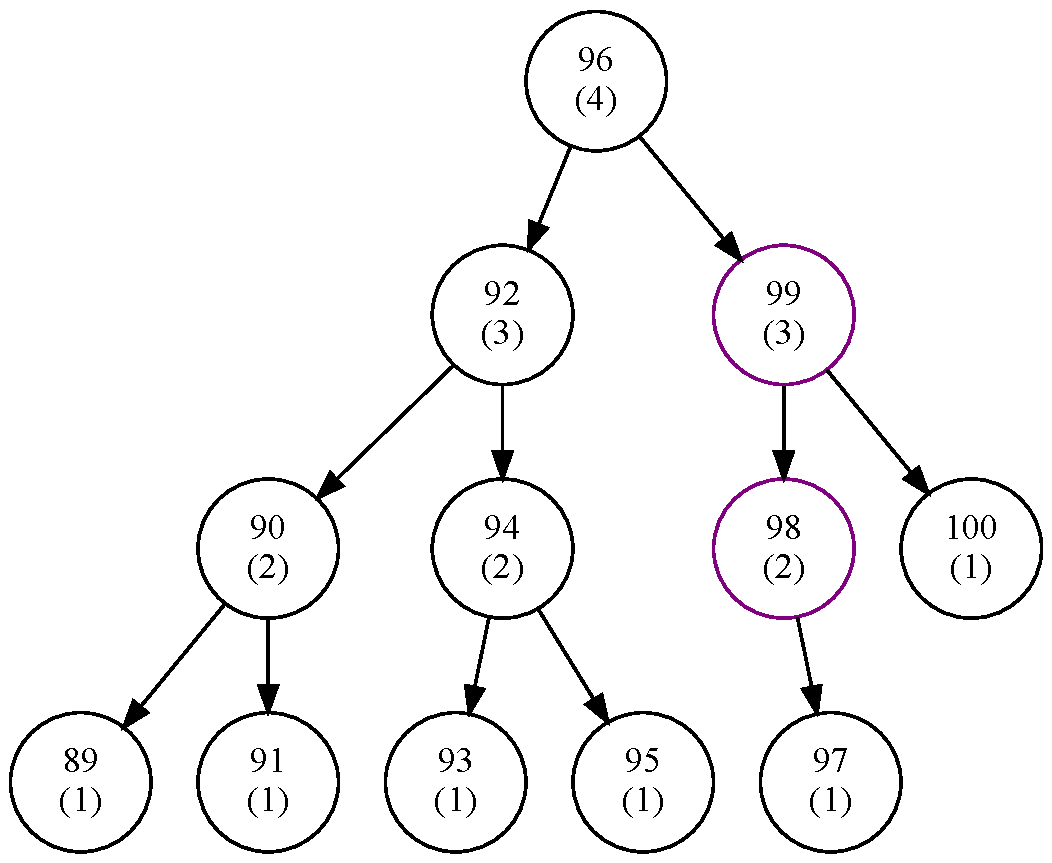
\includegraphics[width = 0.25\textwidth]{img/gv/aufgabe1_6_after.pdf}
    \caption{Nach dem Löschen}
    \label{fig:88after}
\end{figure}

\subsection{Laufzeitmessung}\label{subsec:laufzeitmessung}

Für die Laufzeitmessungen wird die zur Verfügung gestellte Datei \textit{zeitAVLBT} verwendet.
InsertBT, DeleteBT, FindBT, isBT und EqualBT werden hier jeweils für aufsteigende, absteigende und
zufällige Zahlen getestet.
Es wurde über 20 Messungen gemittelt, die Schrittgröße beträgt jeweils 500 Elemente.

In Abbildung~\ref{fig:avl-zeit-kummuliert} ist jeweils die Laufzeit von \textit{FindBT} und
\textit{DeleteBT} kumuliert dargestellt.
Die anderen Methoden wurden hier nicht dargestellt, da deren Laufzeit jeweils nur bis zu 10ms bei
50 Tausend Elementen beträgt, und diese bei einer Messauflösung von 1ms nicht aussagekräftig
sind.
An den Messwerten lässt sich zunächst nicht die Komplexität des Algorithmus festellen,
allerdings lassen sich Aussagen über die relative Laufzeit der jeweiligen Kombinationen festhalten.

In Abbildung~\ref{fig:avl-zeit-el-insert-delete},~\ref{fig:avl-zeit-el-eq-is}
und~\ref{fig:avl-zeit-el-find} sind jeweils die Messungen pro Element dargestellt.
An diesen lässt sich unter anderem die Komplexität des Algorithmus bestimmen.

\paragraph{Löschen vs. Einfügen}
Die erste Auffälligkeit ist, dass das Löschen in allen drei Fällen schneller als das Einfügen ist.
Dies Entspricht nicht den Erwartungen.
Nach diesen müsste das Einfügen schneller als das Löschen sein, da beim Einfügen jeweils maximal
einmal rotiert wird.
Dies wird z.B. an Abbildung~\ref{fig:rebalancing} deutlich:
In beiden Fällen -- dem Left-Right Case und Left-Left Case (und deren gespiegelten Varianten) --
ändert sich die Höhe des Wurzelelementes nach dem Einfügen nicht, diese beträgt weiterhin 1.
\begin{itemize}
    \item Left Right Case: Nach dem Einfügen der 4 beträgt die Höhe 1
    \item Left Left Case: Nach dem Einfügen der 3 beträgt die Höhe 1
\end{itemize}
Beim Löschen ist es hingegen möglich, dass bei jedem Knoten rotiert werden muss.
Somit ist die erwartete Laufzeit vom Löschen besser als die vom Einfügen.

\paragraph{Zufällig vs. Auf- / Absteigend}
Des Weiteren ist sowohl beim Löschen als auch beim Einfügen die Laufzeit bei aufsteigenden Zahlen
ähnlich zu der bei absteigenden Zahlen.
Bei zufälligen Zahlen zeigt der Algorithms jedoch eine bemerkbar schlechtere Laufzeit auf.
Dies ist auch in Abbildung~\ref{fig:avl-zeit-el-find} bei FindBT zu sehen.
Da der Algorithmus bei zufälligen Zahlen nicht langsamer sein sollte als bei sortieren Zahlen, ist
dies wahrscheinlich auf das Generieren der Zufallszahlen zurückzuführen.

Aus Abbildung~\ref{fig:avl-zeit-el-eq-is} lässt sich des Weiteren erkennen, dass die Laufzeit
bei \textit{isBT} und \textit{EqualBT} bei zufälligen und sortierten Zahlen ähnlich ist.
Lediglich \textit{equalBT} zeigt bei zufälligen Zahlen eine etwas höhere Laufzeit auf, dies liegt
jedoch im Rahmen des Messfehlers.
Dies Entspricht den Erwartungen: Da die Bäume in allen Fällen balanciert sind, sollte ein Aufruf
dieser Methoden kein unterschiedliches Verhalten aufzeigen.

\paragraph{Komplexität}
In Abbildung~\ref{fig:avl-zeit-el-insert-delete} wurden für die Bestimmung der Komplexität
bei \textit{InsertBT} und \textit{deleteBT}, jeweils mit zufälligen Zahlen, eine logarithmische
Regression eingezeichnet.
Daran ist zu erkennen, dass die Komplexität des Einfügens und Löschens logaritmisch ist.
Zum Verbessern der Aussagekraft der Messung müsste der Bereich unter 500 Elementen genauer
betrachtet werden, dies ist allerdings durch die hohe Streuung nicht möglich gewesen.

In Abbildung~\ref{fig:avl-zeit-el-find} ist \textit{FindBT} dargestellt.
In dem Bereich von ca. 500 - 5000 Elementen streuen die Werte stark, weswegen sich eine sinnvolle
Regression nicht einzeichnen lässt.
Mit dem bloßem Auge lässt sich allerdings erkennen, dass die Laufzeit von \textit{FindBT} bei
zufälligen
Zahlen einen logaritmischen Trend aufzeigt.
Bei sortierten Zahlen lässt sich im Gegensatz nicht sagen, ob der Graph logarithmisch oder konstant
ist.
Letzteres lässt sich allerdings ausschließen, da aus dem Entwurf bekannt ist, dass bei
\textit{FindBT} über
den Baum gelaufen wird und somit keine konstante Komplexität vorliegen kann.
Um dies zu bestätigen, müsste auch hier die Laufzeit für Elementanzahlen unter 500
durchgeführt werden.

\begin{figure}[hbt]
    \centering
    \subfloat[\centering Kumuliert]{
        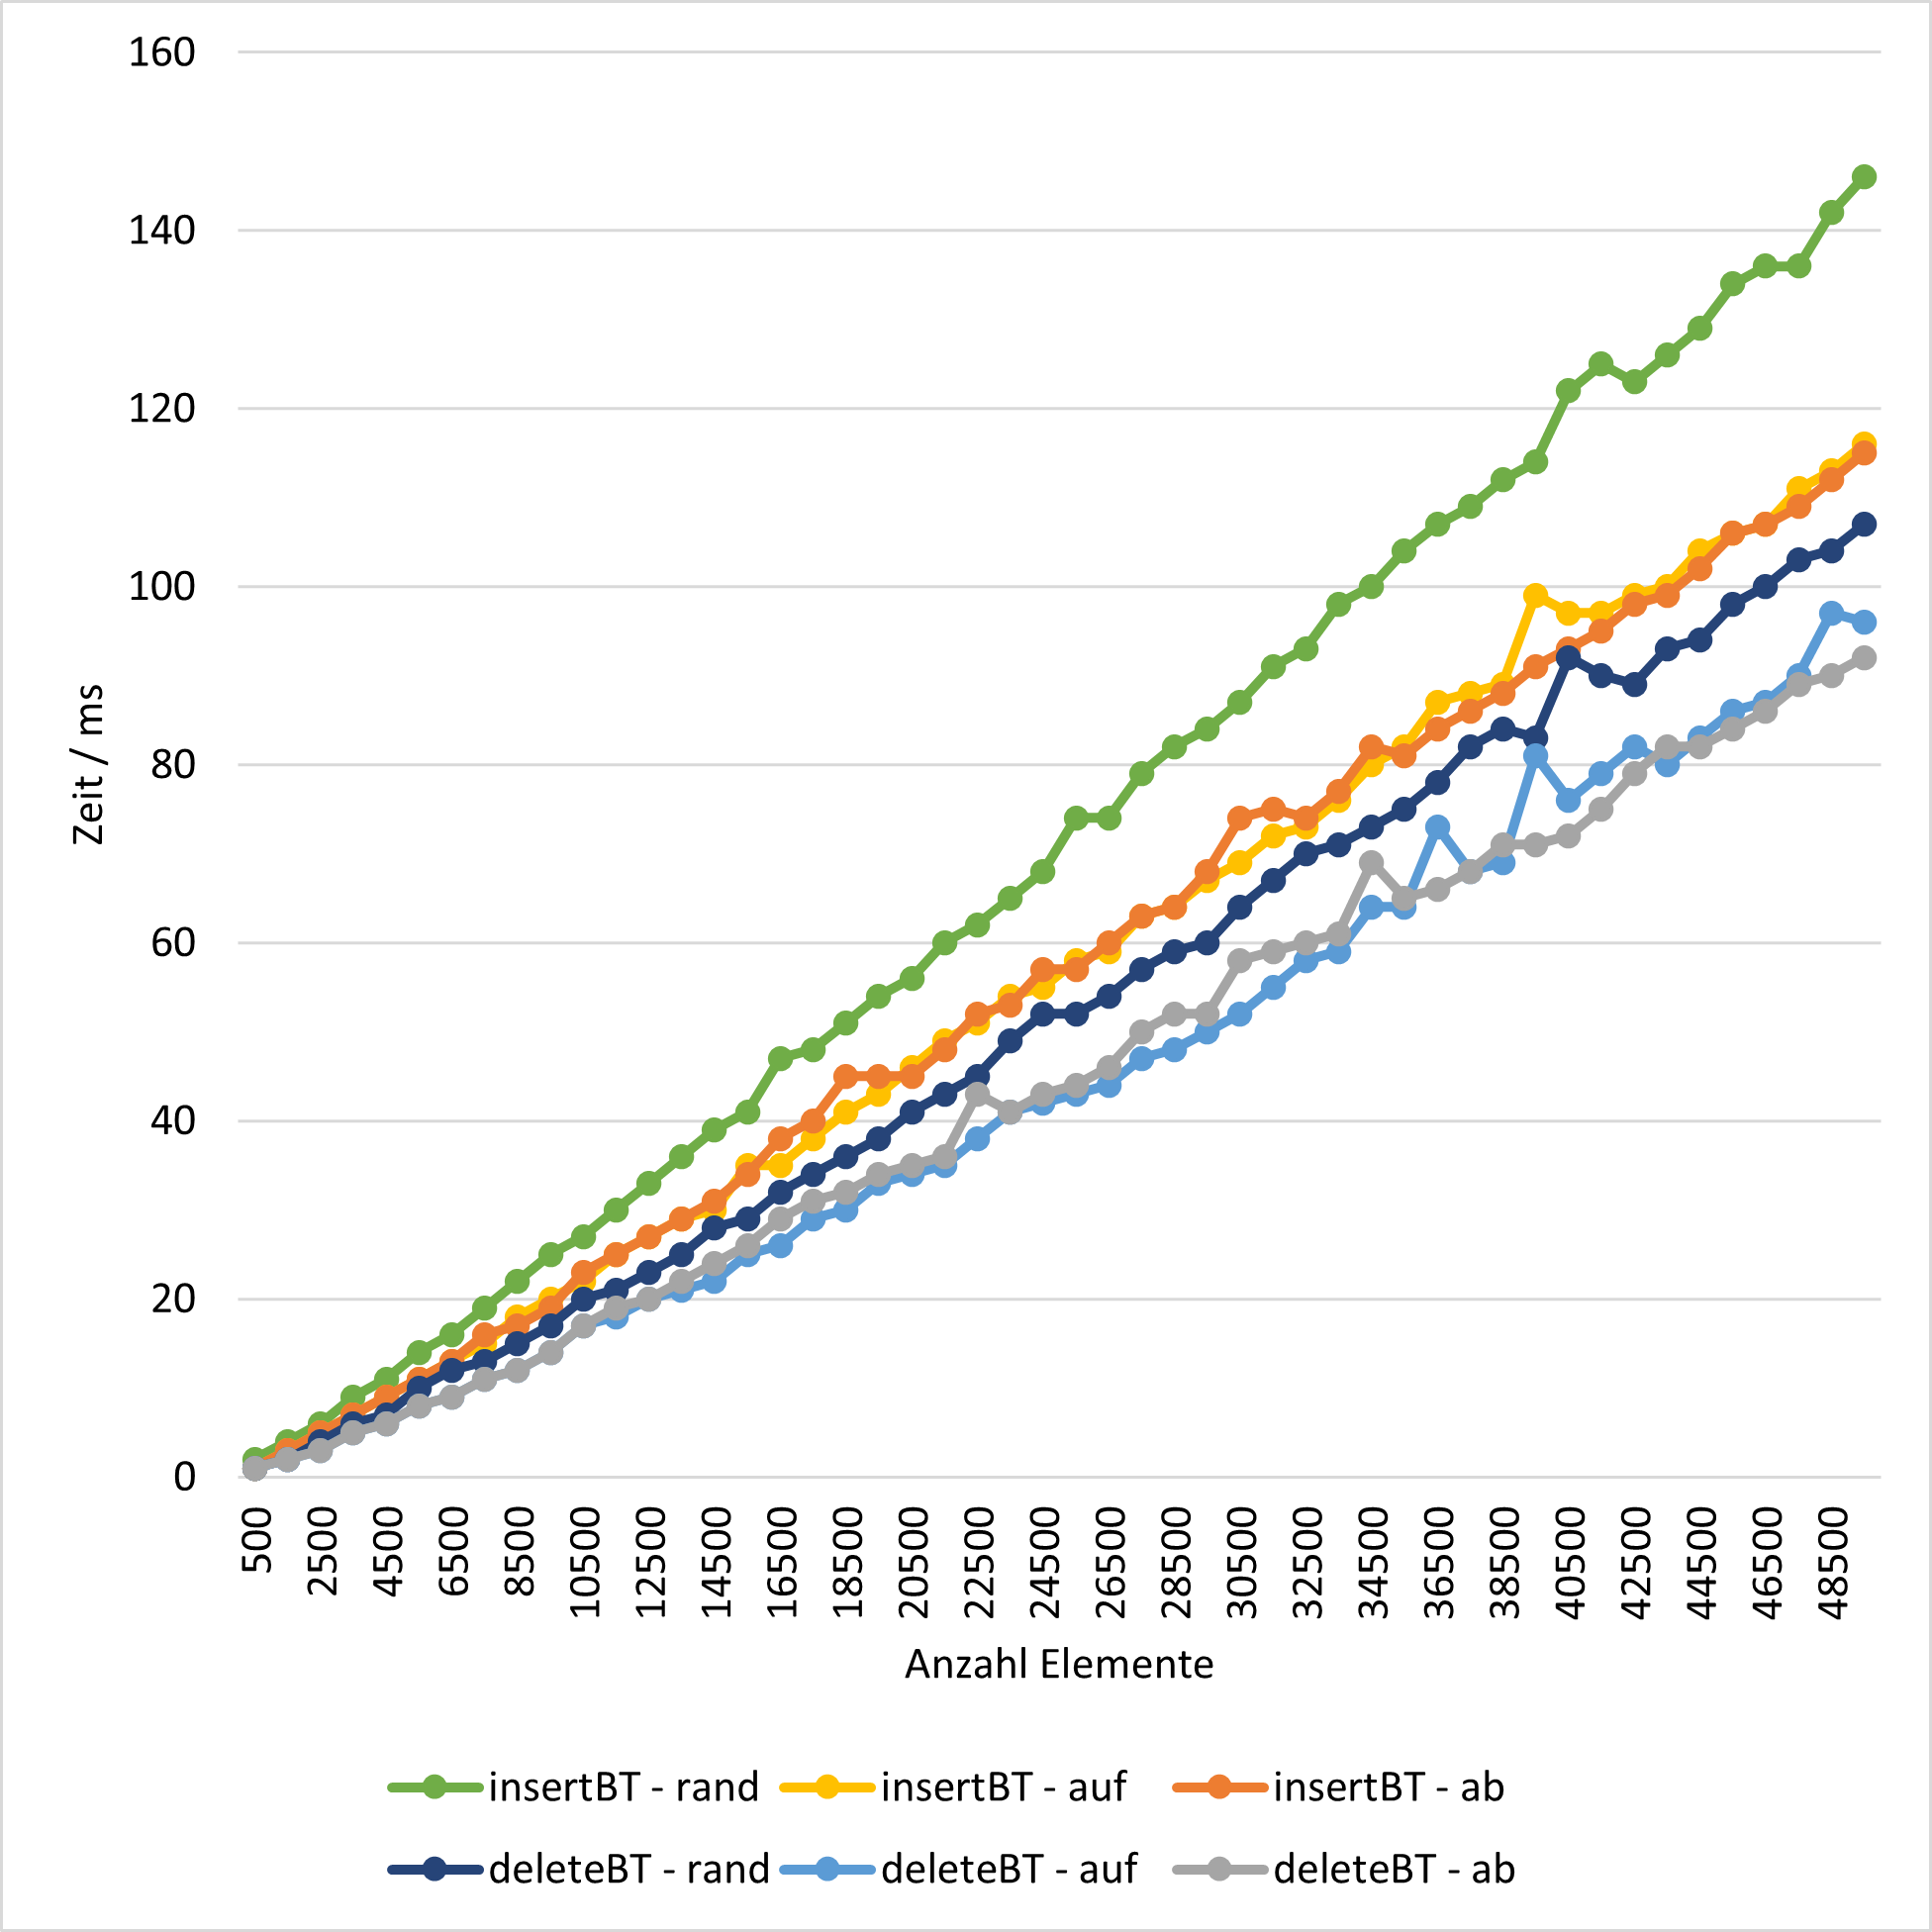
\includegraphics[width = 0.45\textwidth]
        {img/excel/avl1.png}\label{fig:avl-zeit-kummuliert}}
    \qquad
    \subfloat[\centering Pro Element - DeleteBT und InsertBT]{
        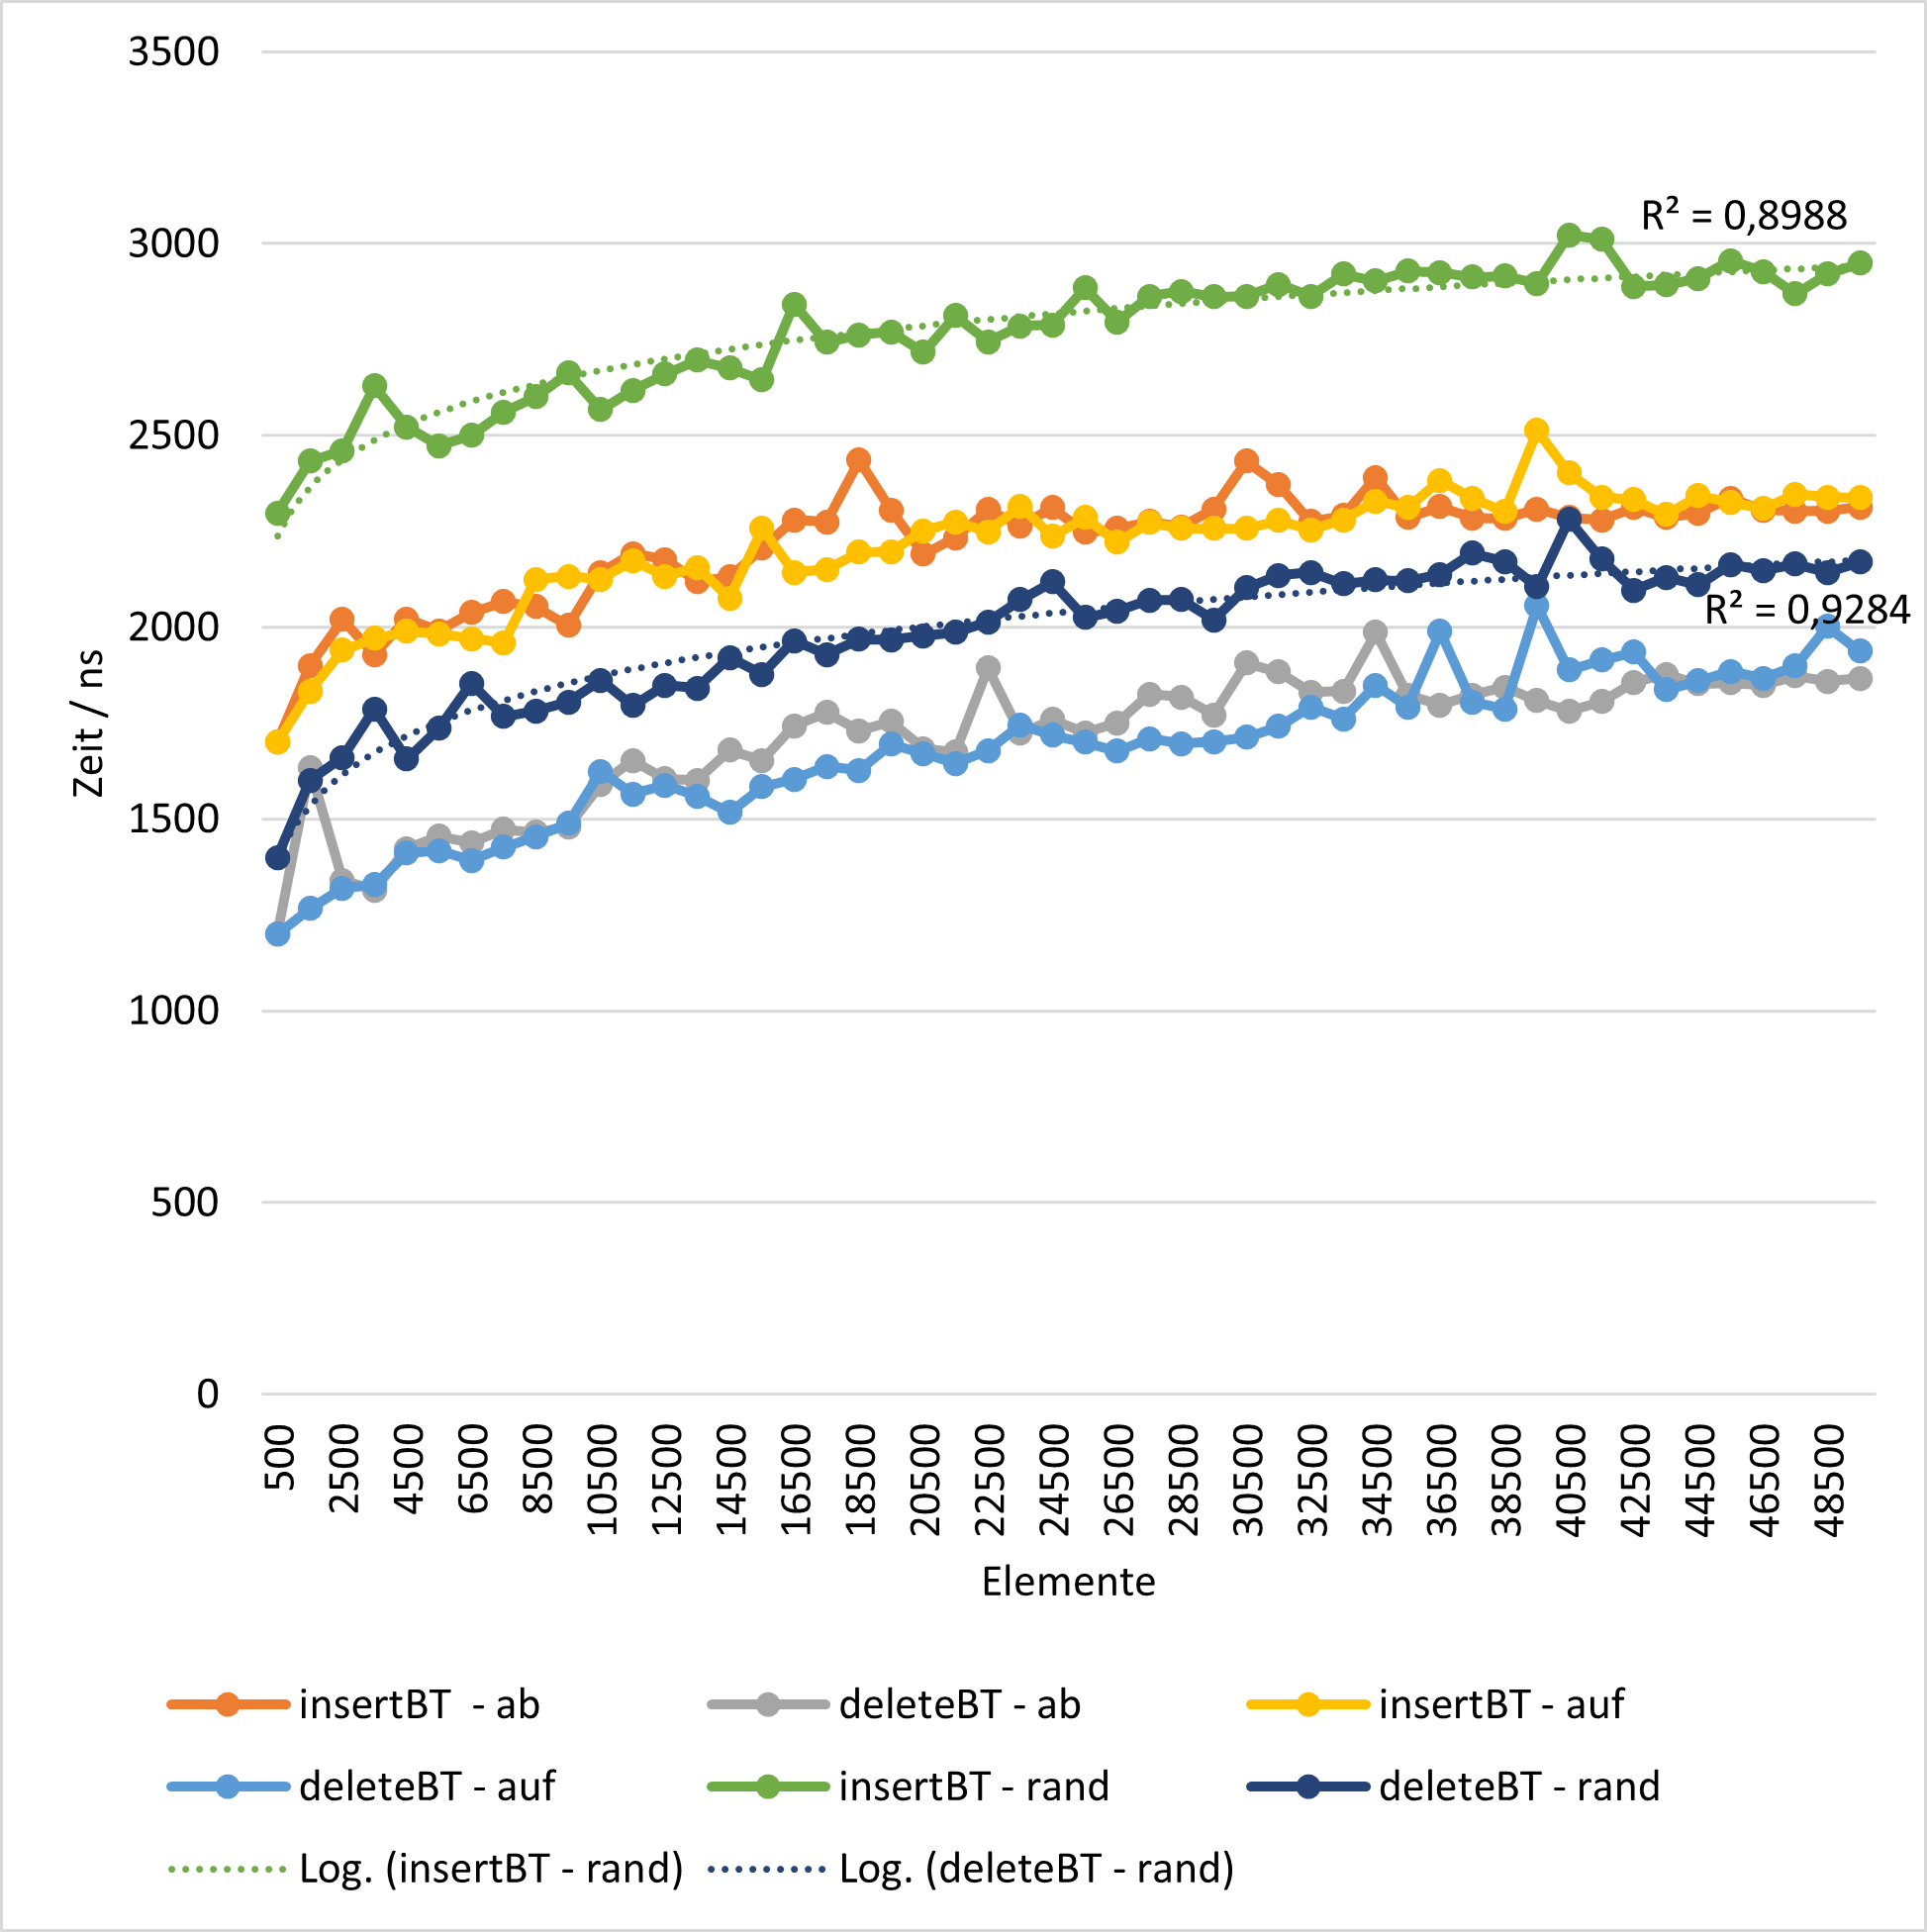
\includegraphics[width = 0.45\textwidth]
        {img/excel/avl1_el.png}\label{fig:avl-zeit-el-insert-delete}}
    \qquad
    \subfloat[\centering Pro Element - EqualBT und IsBT]{
        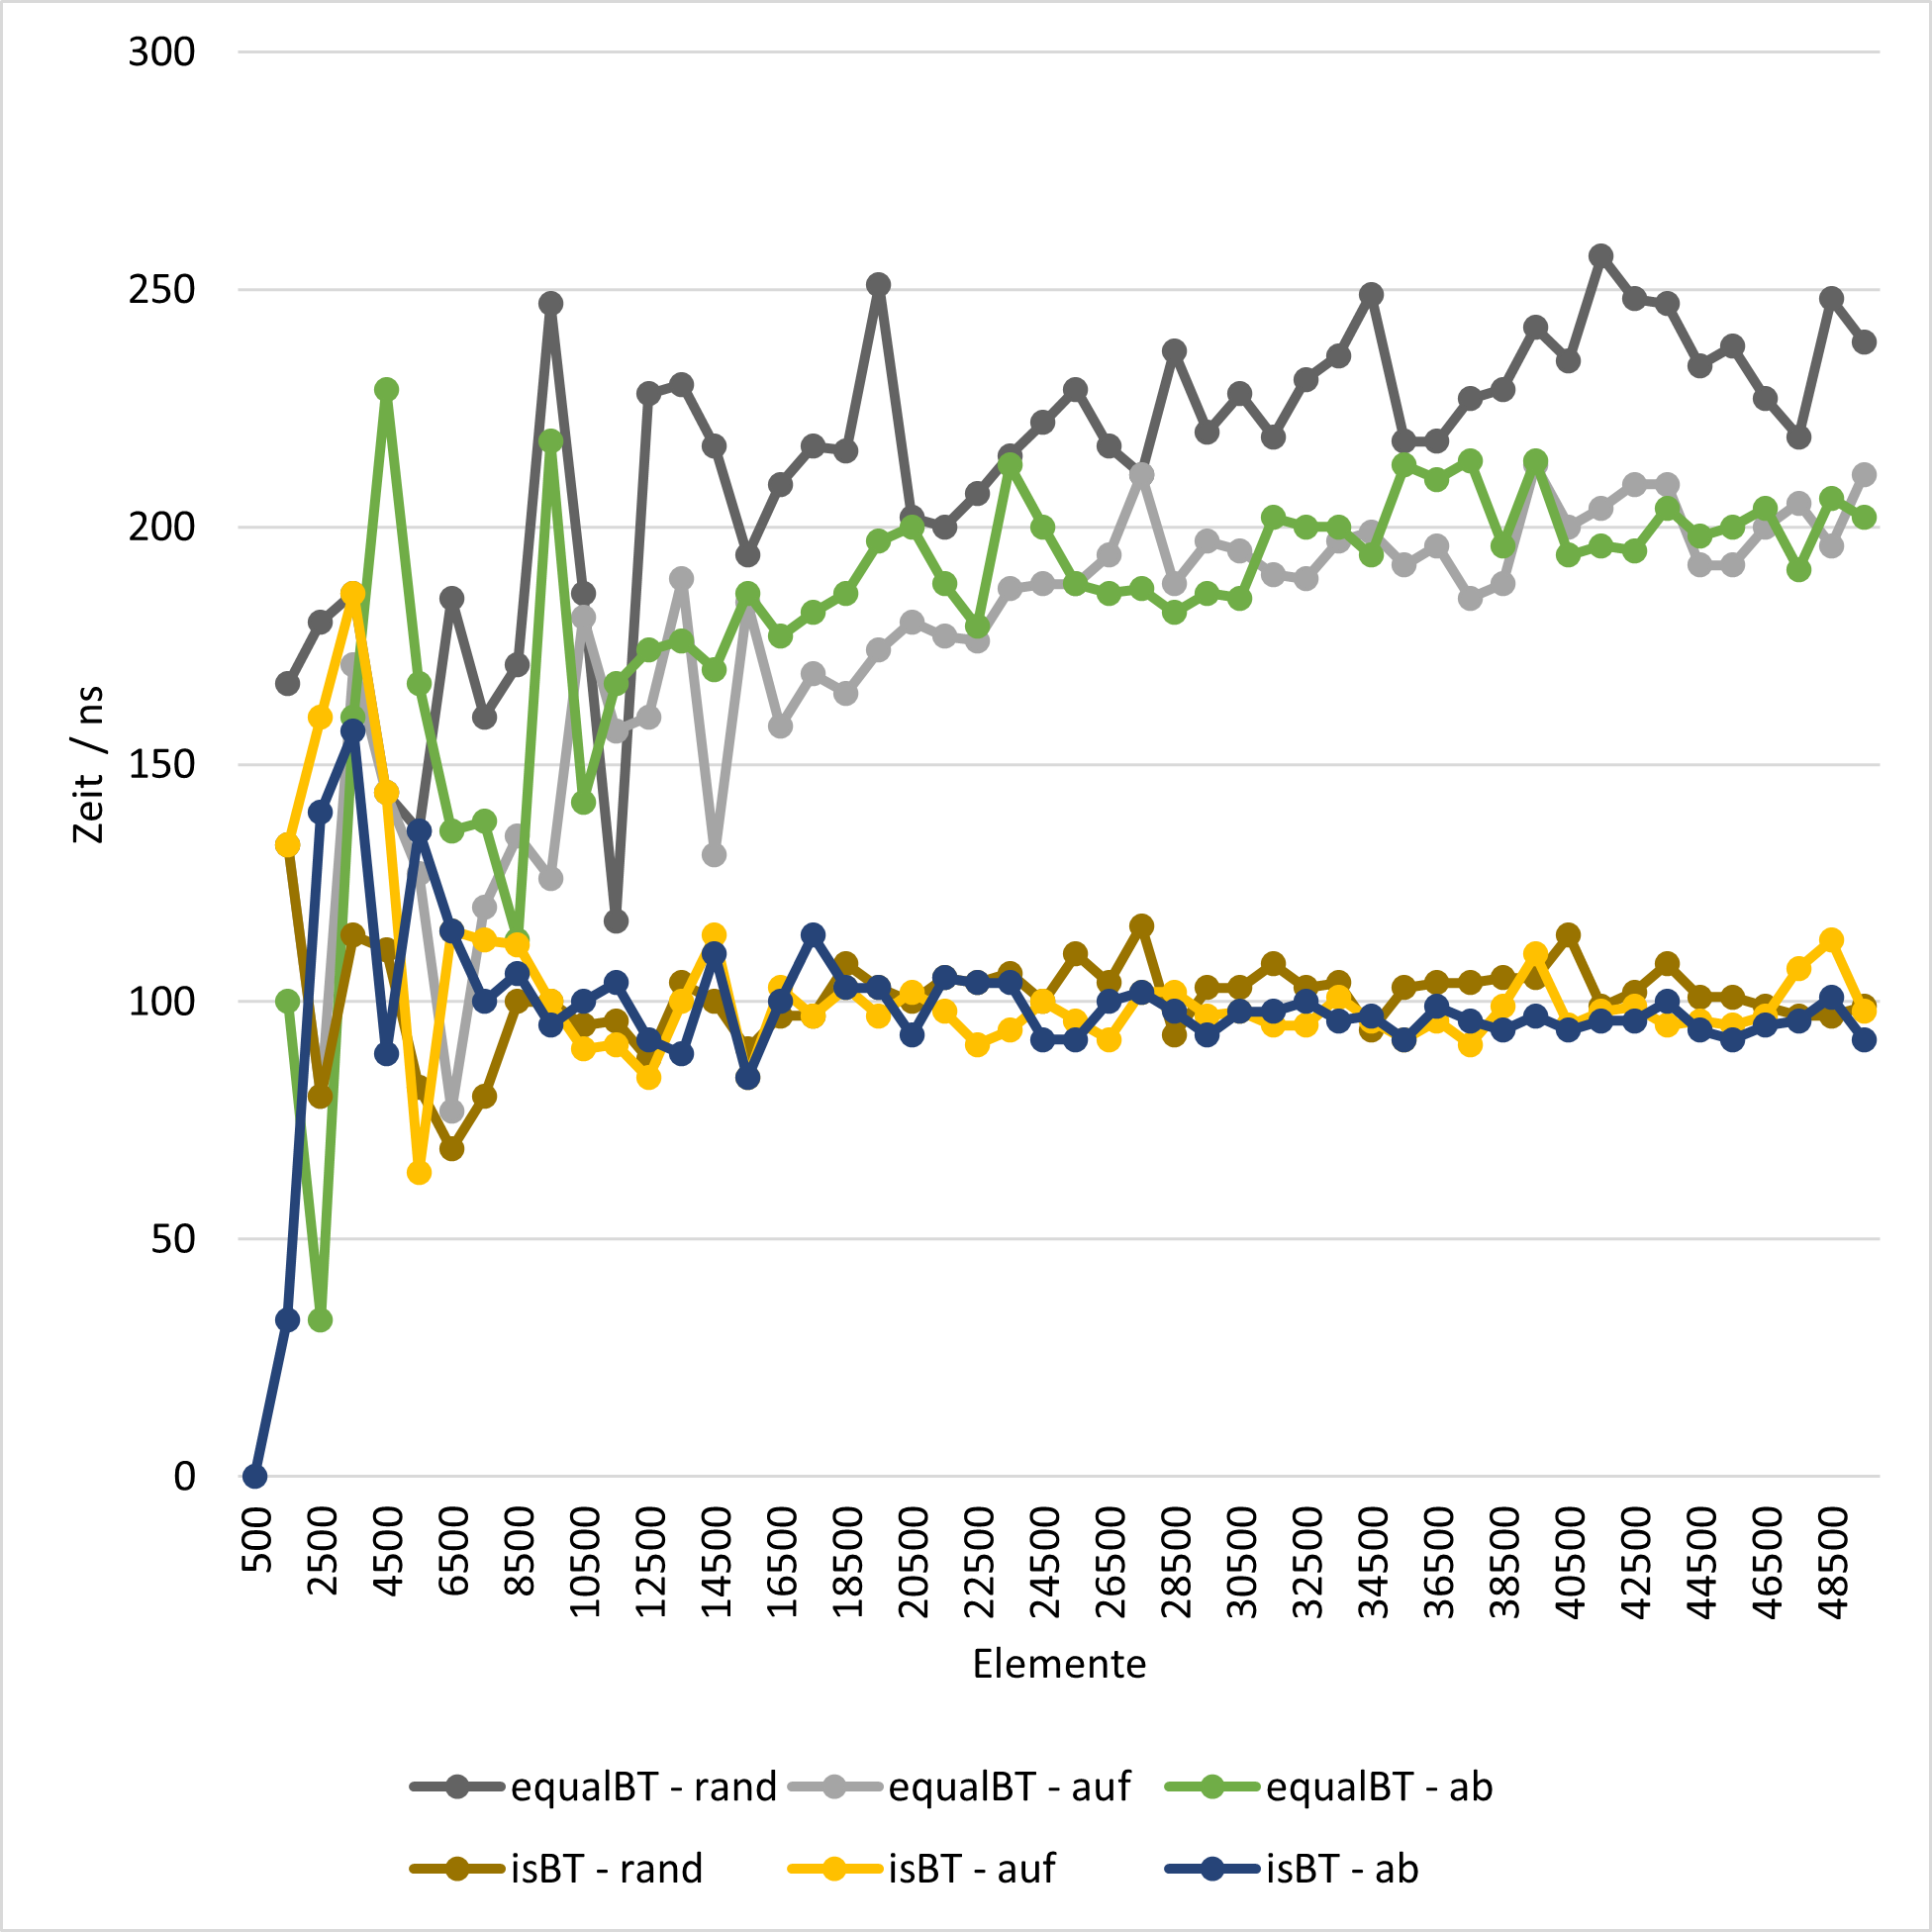
\includegraphics[width = 0.45\textwidth]
        {img/excel/avl2_el.png}\label{fig:avl-zeit-el-eq-is}}
    \qquad
    \subfloat[\centering Pro Element - FindBT]{
        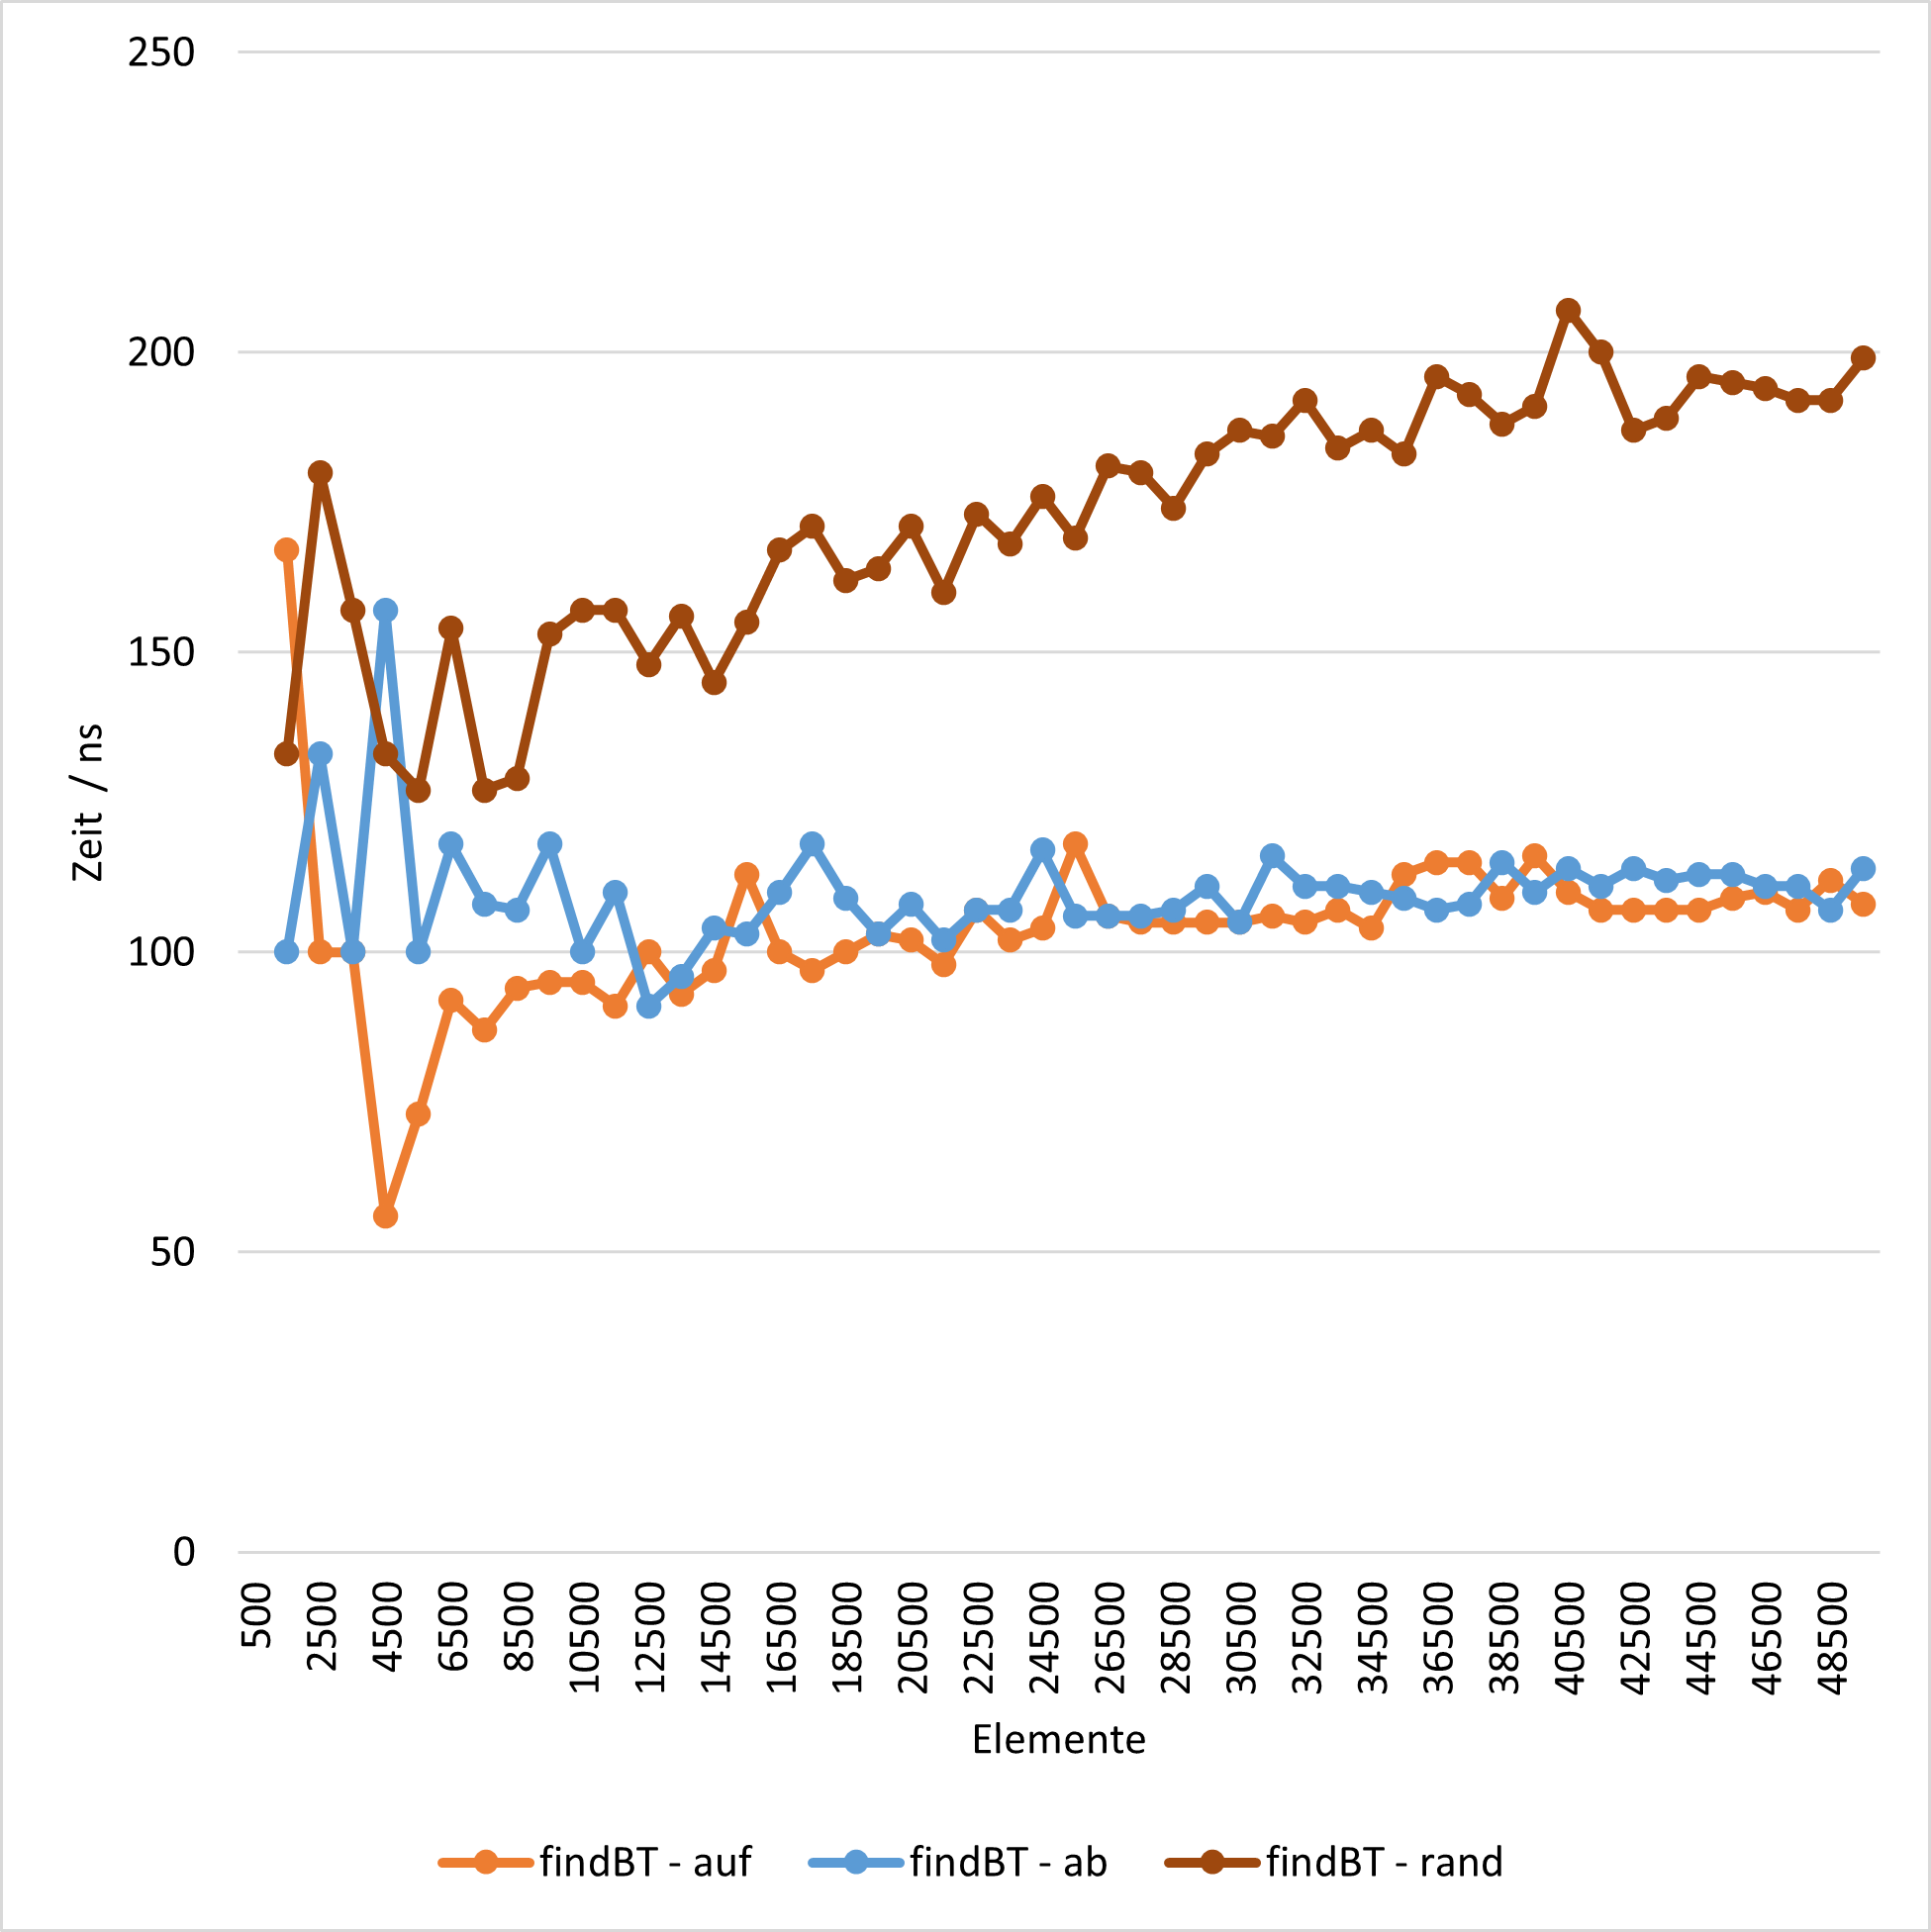
\includegraphics[width = 0.45\textwidth]
        {img/excel/avl3_el.png}\label{fig:avl-zeit-el-find}}
    \caption{Zeitmessungen AVL-Baum}
    \label{fig:avl_zeit}
\end{figure}

\FloatBarrier




    \section{Splay Tree}\label{sec:splay-tree}
    \subsection{Algorithmus}\label{subsec:splay-algorithmus}
Ein Splay-Tree ist ein Binärbaum, der beim Einfügen und Suchen von Elementen, diese jeweils an
die Wurzel befördert.
Dieser Vorgang wird Splaying gennant.

\subsubsection{Splaying}
Ähnlich wie beim AVL-Baum wird wieder ein Knoten als Wurzel betrachtet.
Zunächst wird das gesuchte Element an diese Wurzel gebracht.
Dieser Prozess wird anschließend rekursiv auf die verbleibenden Knoten über der Wurzel angewendet,
bis das Element an der Wurzel des kompletten Baumes steht.

Es wird zwischen 3 Fällen unterschieden, die durch den Pfad von der Wurzel zu dem nach oben
zu befördernden Elementes definiert sind.
Alle Fälle haben jeweils ein symmetrisches Paar.
In Abbildung~\ref{fig:splayinCase} ist jeweils eines der Paare dargestellt.
In Klammern ist der symmetrische Fall angegeben.
Die Wurzel \verb|x| ist dabei jeweils die, die nach oben befördert werden soll.
Der Vorgang wird im Entwurf der Methode \nameref{par:splay} (Abschnitt~\ref{par:splay})
weiter ausgeführt.
%\begin{enumerate}
%    \item Zig-Zag: L/L oder R/R
%    \item Zig-Zig: L/R oder R/L
%    \item Zig: L oder R
%\end{enumerate}

\begin{figure}[hbt]
    \centering
    \subfloat[\centering Zig Zig: L/L (R/R)]{
        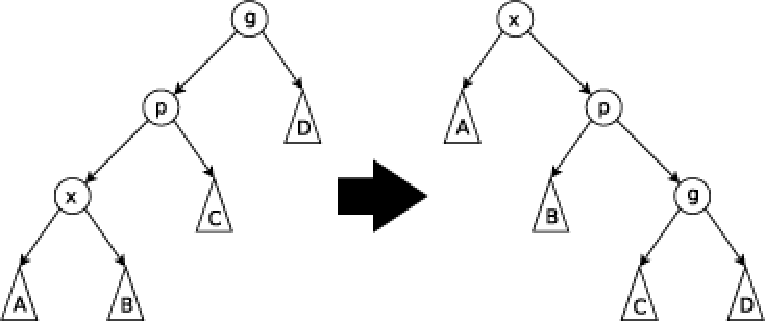
\includegraphics[width = 0.45\textwidth]{img/external/zigzig}\label{fig:splayingCase-zig-zig}}
    \qquad
    \subfloat[\centering Zig Zag: L/R (R/L)]{
        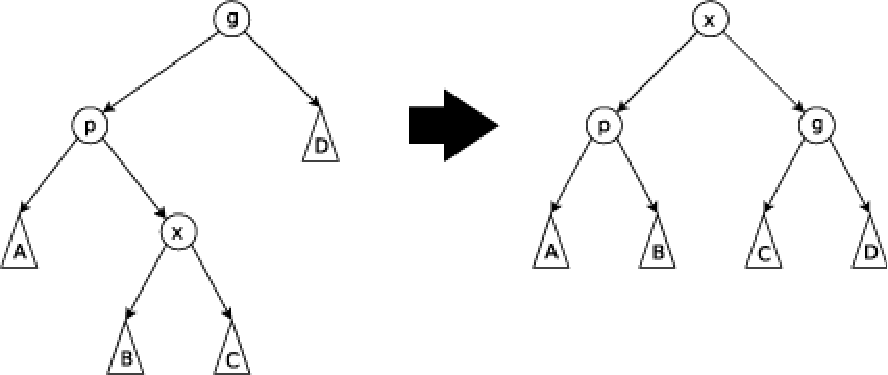
\includegraphics[width = 0.48\textwidth]{img/external/zigzag}\label{fig:splayingCase-zig-zag}}
    \qquad
    \subfloat[\centering Zig: L (R)]{
        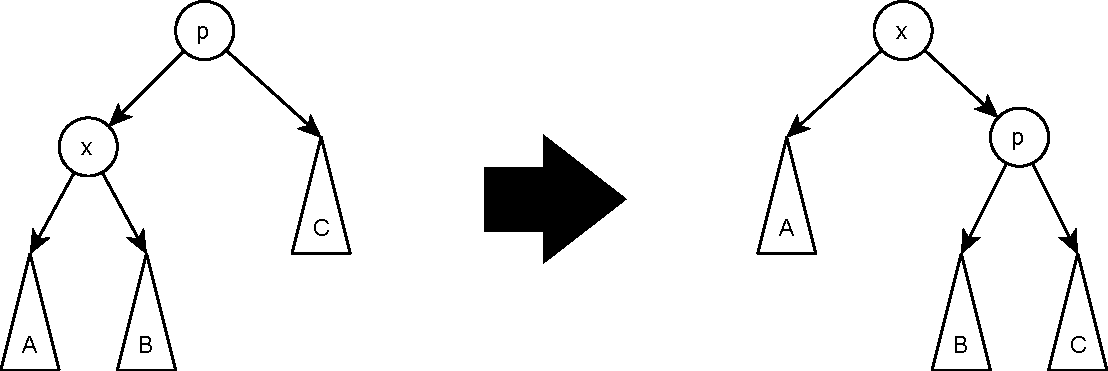
\includegraphics[width = 0.52\textwidth]{img/external/zig}\label{fig:splayingCase-zig}}
    \caption{Splaying Vorgang}\label{fig:splayinCase}
\end{figure}

\subsection{Entwurf}\label{subsec:splay-entwurf}

\subsubsection{InitBT, IsEmptyBT, EqualBT, PrintBT}
Wie beim AVL-Baum kann auch hier die Implementation des Binärbaumes verwendet werden.
Lediglich InitBT wird wieder um das Zurücksetzen der Counter erweitert.
PrintBT ist identisch zu der in Abschnitt~\ref{par:printBT} beschrieben Methode.

\subsubsection{IsBT}
Bei dem AVL-Baum wurde \nameref{par:avl-isBT} um das Überprüfen der AVL-Bedingung erweitert.
So konnte die korrekte Arbeitsweise des AVL-Baumes sichergestellt werden.
Bei dem Splay-Tree lässt sich die Korrektheit vom Splaying jedoch nicht überprüfen, da die
Datenstruktur selber keine Informationen über die Zugriffe auf Elemente speichert.
In \verb|IsBT(BTree)| werden also lediglich die Voraussetzungen des Binärbaumes überprüft,
somit kann die Implementation vom Binärbaum übernommen werden.

\subsubsection{FindBT}\label{par:splay-findBT}
Beim Finden eines Elementes wird dieses an die Wurzel des Baumes befördert.
Dafür wird zunächst top-down das gesuchte Element gefunden, wobei der Pfad
bottom-up hoch gegeben wird.
Als Erstes wird \verb|HERE|, danach \verb|L| oder \verb|R| zurückgegeben.
Beim zweiten Schritt ist das gesuchte Element zwei Elemente entfernt, kann also über zwei
Kanten erreicht werden.
Nun wird die entsprechende Doppelrotation durchgeführt, dies wird in die \nameref{par:splay}
Methode ausgelagert.
Das gesuchte Element steht jetzt an dem Knoten, der gerade als Wurzel betrachtet wird, somit wird
als Pfad \verb|HERE| zurückgegeben.
Dies wird rekursiv fortgeführt, bis die Wurzel des Baumes erreicht wird.
Der Vorgang ist in Abbildung~\ref{fig:splayFind} dargestellt.
\begin{figure}[hbt]
    \centering
    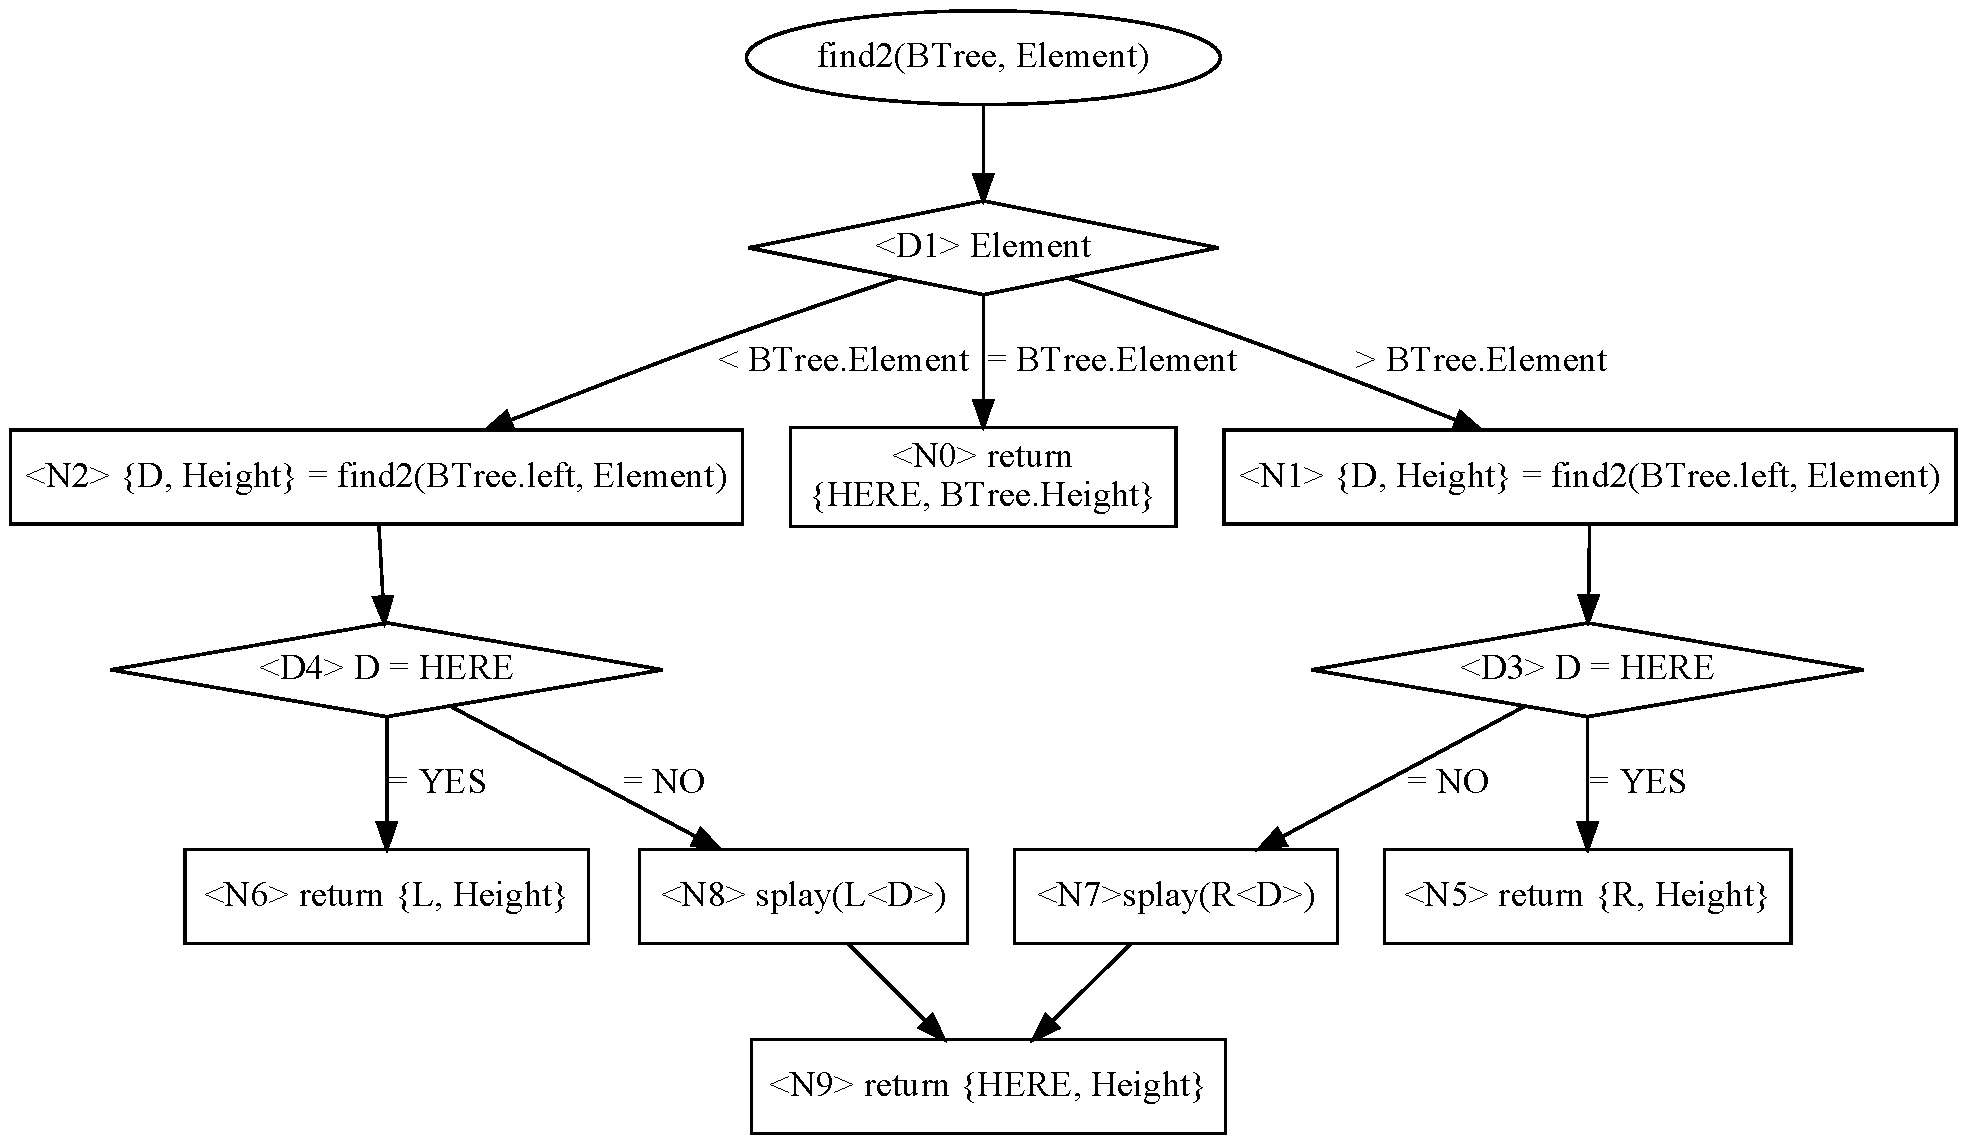
\includegraphics[width=0.8\textwidth]{img/gv/splayFind2}
    \caption{FindBT}
    \label{fig:splayFind}
\end{figure}

In der Abbildung ist der Fall, dass das gesuchte Element nicht im Baum vorhanden ist, präteriert.
Hierfür wird der Pfad als \verb|NOTFOUND| zurückgegeben.
Falls bei der Überprüfung dessen \verb|NOTFOUND| vorliegt, wird wiederum \verb|HERE|
zurückgegeben, was dazu führt, dass das zuletzt aufgerufene Element zur Wurzel wird \verb|<R1>|.

Da immer zwei Nachfolger betrachtet werden, ist es möglich, dass am Ende das gesuchte Element
am linken oder rechtem Kind vom Wurzelknoten steht.
Um dies zu überprüfen, wird die eben beschriebene Methode in eine Wrapper-Methode umhüllt.
Dort kann getestet werden, ob am Ende \verb|HERE| zurückgegeben wurde.
Falls dies der Fall ist, wird ein Zig (Einfachrotation) ausgeführt.
Anschließend steht das gesuchte Element an der Wurzel.
Dies ist in Abbildung~\ref{fig:splayFind2} dargestellt.
\begin{figure}[hbt]
    \centering
    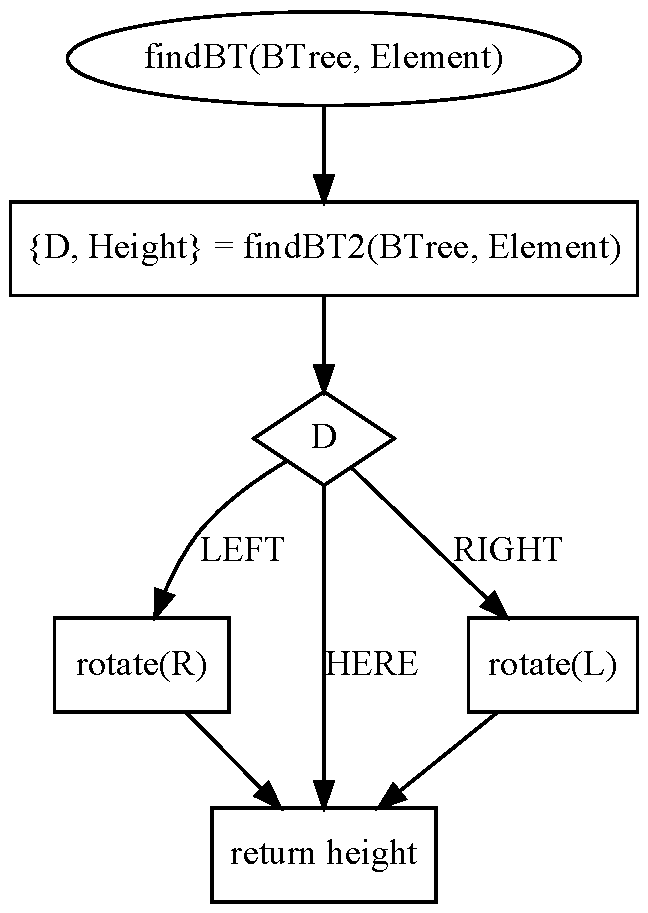
\includegraphics[width=0.3\textwidth]{img/gv/splayFind}
    \caption{FindBT Wrapper}
    \label{fig:splayFind2}
\end{figure}
Diese Operation ist in allen Methoden zu implementieren und wird in den Entwurf dieser nicht
explizit betrachtet.

\subsubsection{Splay}\label{par:splay}
Die Splay Methode bekommt einen Baum und einen Pfad \(P \in \{LL, RR, LR, RL\}\) übergeben,
welcher angibt, welcher Splaying Fall vorliegt.
Es wird eine Fallunterscheidung über den Pfad gemacht, welche die Abfolge der Rotationen bestimmt.
Diese sind wie beim AVL Baum zu implementieren.
\begin{itemize}
    \item LL → Rechtsrotation auf Wurzel → Rechtsrotation auf neue Wurzel. \verb|<R1>|
    \item RR → Linksrotation auf Wurzel → Linksrotation auf neue Wurzel. \verb|<R2>|
    \item RL → Rechtsrotation auf rechtes Kind → Linksrotation auf Wurzel. \verb|<R3>|
    \item LR → Linksrotation auf linkes Kind → Rechtsrotation auf Wurzel. \verb|<R4>|
\end{itemize}

\subsubsection{FindTP}
Alternativ kann beim Finden eines Elementes dieses nur um einen Knoten nach oben bewegt werden.
Zunächst wird das Element gefunden, anschließend eine Zig-Operation durchgeführt.
Um dies zu realisieren, wird, sobald das gesuchte Element gefunden wurde, ein Flag zurückgegeben,
welches signalisiert, dass rotiert werden soll \verb|<R1>|.
Wenn beim Überprüfen des Rückgabewertes das Flag gesetzt ist, wird in die entsprechende Richtung
rotiert \verb|<R2>|.
Somit wird das Element nur um eine Ebene nach oben gegeben, anschließend nicht mehr zurückgegeben
wird \verb|<R3>|.
Falls ein Element nicht gefunden wird, wird \verb|NOTFOUND| zurückgegeben \verb|<R4>|, beim
Überprüfen des Pfades wird daraufhin \verb|HERE| zurückgeben \verb|<R5>|, was dazu führt, dass
wieder genau einmal rotiert wird.

\subsubsection{InsertBT}
Beim Einfügen eines Elementes wird dieses an die Wurzel befördert.
Dies kann dadurch realisiert werden, dass das Element zunächst wie bei einem Binärbaum
eingefügt, anschließend mithilfe von \nameref{par:splay-findBT} an die Wurzel befördert wird.
Diese Implementation hat den Nachteil, dass der Baum insgesamt zweimal durchlaufen wird.
Zur Optimierung werden, beide Schritte in einem Durchlauf durchgeführt: Zunächst top-down
das Element einfügen \verb|<R1>|, dann, mithilfe von Rotationen, bottom-up das Element zur Wurzel
bringen \verb|<R2>|.
Dabei ist letzteres wie bei \nameref{par:splay-findBT} zu realisieren,
die Höhe muss dabei nicht zurückgegeben werden.
Außerdem muss das \verb|NOTFOUND| nicht zurückgegeben werden, da dieser Fall hier nicht auftritt.
Stattdessen wird nach dem Einfügen \verb|HERE| zurückgegeben, damit dieses Element gesplayt wird
\verb|<R3>|.

\subsubsection{DeleteBT}
Bei deleteBT wird ein Element als Erstes mit \nameref{par:splay-findBT} an die Wurzel befördert
\verb|<R1>|.
Dieses wird gelöscht, nun bleiben zwei Teilbäume, übrig, welche mit \nameref{par:joinbt} zu einem
zusammengeführt werden \verb|<R2>|.
Wenn ein Element nicht gefunden wird, wird das zuletzt besuchte Element gesplayt, dies wird wie
in \nameref{par:splay-findBT} (Abschnit~\ref{par:splay-findBT}) realisiert.

\subsubsection{JoinBT}\label{par:joinbt}
Um zwei Bäume zu einem zusammenzuführen wird zunächst das größte Element des linken Teilbaumes
gesplayt \verb|<R1>|, somit hat die neue Wurzel kein rechtes Kind, da es das größte Element des
Baumes ist.
Der rechte Teilbaum wird jetzt als rechtes Kind der neuen Wurzel gesetzt \verb|<R2>|.

\subsection{Aufgaben}\label{subsec:aufgaben2}

\subsubsection{Aufgabe 2.5 - Analysieren beispielhafter Bäume}
Beispielhafte Bäume werden mit der zur verfügung gestellten Methode\\
\verb|analysesBT:test(<Anzahl Elemente>)| analysiert.

\subparagraph{100 Elemente}
Ein Aufruf mit 100 Elementen ergibt folgende Ausgabe:
\begin{verbatim}
> analysesBT:test(100).
Ausgaben beziehen sich auf die Rahmenbedingungen von AVL-Bäumen.
Bei gegebener Höhe 17:
         minimale Anzahl Knoten: 4180.
         maximale Anzahl Knoten: 131071
Bei gegebener Anzahl an Knoten 100:
         minimale Höhe: 6.
         maximale Höhe: 9
Durchschnittliche Balancefehler: 2.19
         maximaler Balancefehler: 10.
\end{verbatim}

\subparagraph{1000 Elemente}
Ein Aufruf mit 1000 Elementen ergibt folgende Ausgabe:
\begin{verbatim}
> analysesBT:test(1000).
Ausgaben beziehen sich auf die Rahmenbedingungen von AVL-Bäumen.
Bei gegebener Höhe 25:
         minimale Anzahl Knoten: 196417.
         maximale Anzahl Knoten: 33554431
Bei gegebener Anzahl an Knoten 1000:
         minimale Höhe: 9.
         maximale Höhe: 14
Durchschnittliche Balancefehler: 1.97
         maximaler Balancefehler: 18.
\end{verbatim}

An den Ausgaben ist zu erkennen, dass die Bäume im Vergleich zu AVL-Bäumen deutlich schlechter
balanciert sind.
Bei beiden Ausgaben ist der durchschnittliche Balancefehler ca. 2, wobei dieser bei den
AVL-Bäumen nur bei ca. 0.3 lag.
Außerdem überschreitet die Höhe vom Splay-Tree im ersten Beispiel die maximale Höhe eines AVL-Baumes
um 100 Prozent.
Hierdurch wird ersichtlich, dass ein Splay-Tree für Zufällige Lese- und Schreiboperationen eine
schlechtere Charakteristik aufzeigt.

\subsubsection{Aufgabe 2.6 - Prüfen der Strategie anhand von Bildern}
Zum Prüfen der Korrektheit der Strategie werden kleine Bäume mithilfe von printBT ausgegeben.
In Abbildung~\ref{fig:splay-base} ist der Ausgangsbaum dargestellt.
Alle folgenden Operationen werden auf diesem Baum ausgeführt.

\paragraph{Im Baum vorhandene Elemente}
In Abbildung~\ref{fig:splay-del4} wurde die 4 gelöscht.
Der Vaterknoten der 4 ist die 3 gewesen, somit wurde diese gesplayt und steht nun an der Wurzel.

In Abbildung~\ref{fig:splay-findbt4} wurde die \verb|FindBT(4)| auf den Ausgangsbaum angewandt,
die 4 wurde gesplayt und steht jetzt an der Wurzel.

In Abbildung~\ref{fig:splay-findtp4} wurde die \verb|FindTP(4)| auf den Ausgangsbaum angewandt.
Die 4 wurde um eine Position gesplayt.

In Abbildung~\ref{fig:splay-insert10} wurde die 10 eingefügt, diese wurde an die Wurzel gesplayt.

\begin{figure}[hbt]
    \centering
    \subfloat[\centering Ausgangsbaum]{
        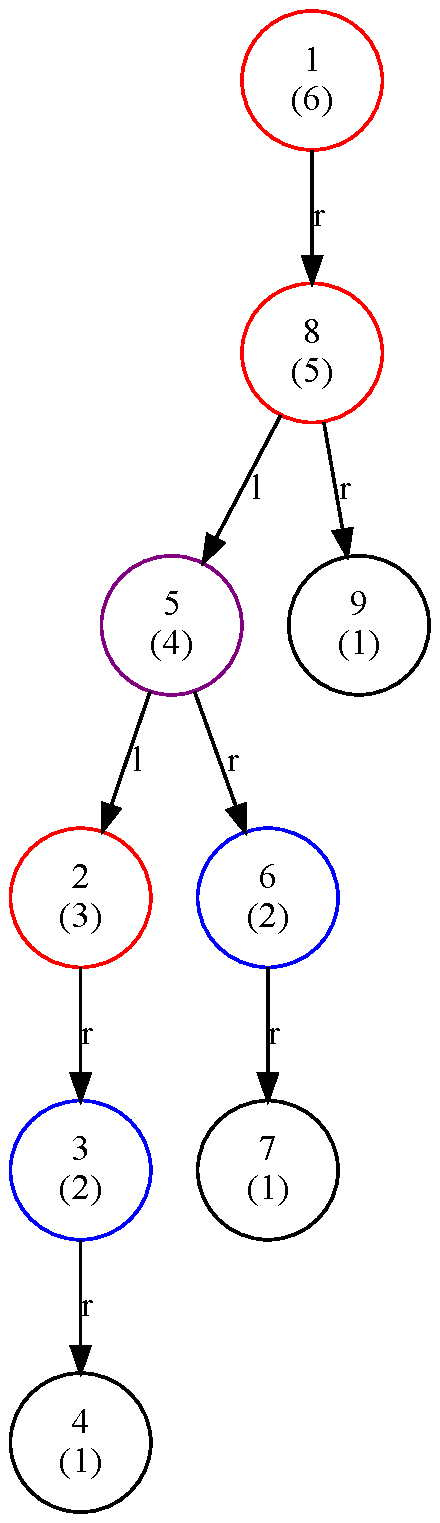
\includegraphics[scale = 0.32]{img/gv/aufg2_6}\label{fig:splay-base}}
    \qquad
    \subfloat[\centering Delete 4]{
        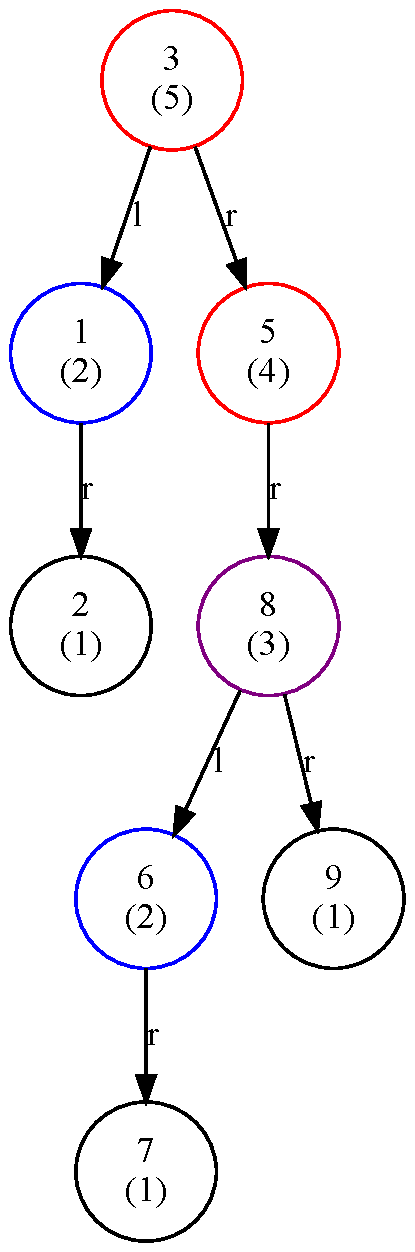
\includegraphics[scale = 0.32]{img/gv/aufg2_6_Delete4}\label{fig:splay-del4}}
    \qquad
    \subfloat[\centering FindBT 4]{
        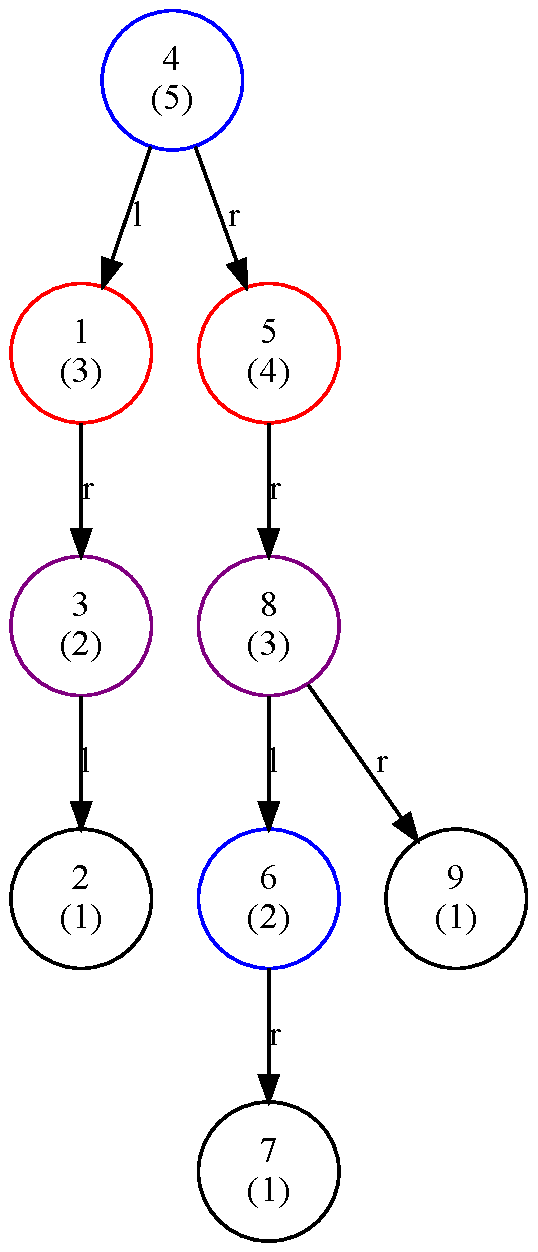
\includegraphics[scale = 0.32]{img/gv/aufg2_6_FindBT4}\label{fig:splay-findbt4}}
    \qquad
    \subfloat[\centering FindTP 4]{
        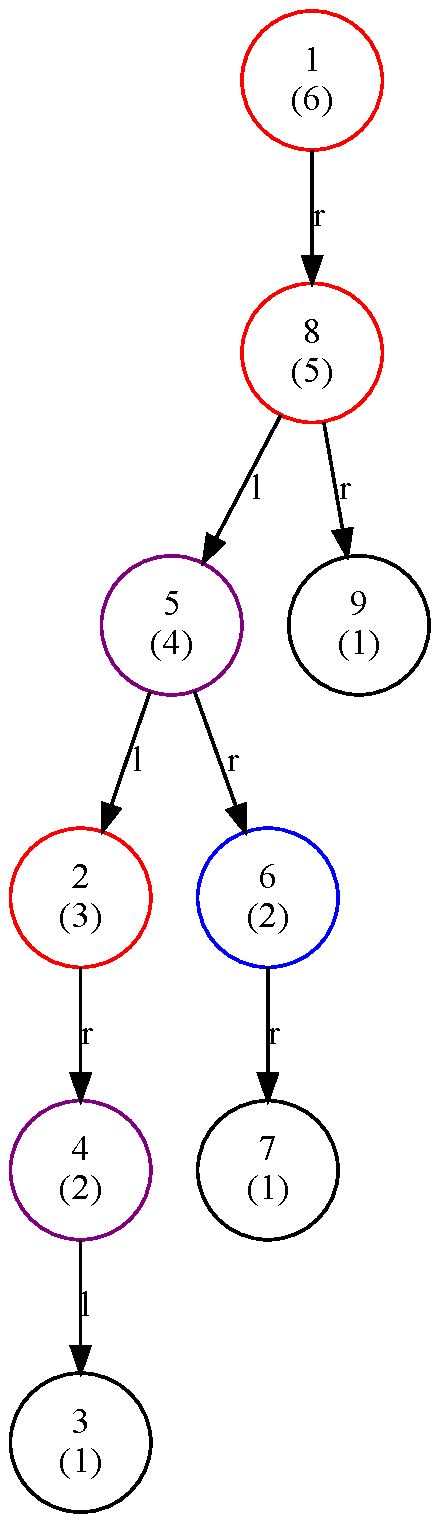
\includegraphics[scale = 0.32]{img/gv/aufg2_6_FindTP4}\label{fig:splay-findtp4}}
    \caption{Bilder der Splaying-Strategie - vorhandene Elemente}\label{fig:splay}
\end{figure}

\paragraph{Im Baum nicht vorhandene Elemente}

In Abbildung~\ref{fig:splay-findbt99} und Abbildung~\ref{fig:splay-delete99} wurde jeweils die
99 gesucht bzw gelöscht.
Da die 99 nicht existiert wurde der Vaterknoten (9) gesplayt und steht anschließend an der Wurzel.

In Abbildung~\ref{fig:splay-findtp99} wurde die \verb|FindTP(99)| auf den Ausgangsbaum angewandt.
Hier wurde die 9 um eine Position gesplayt.

\begin{figure}[hbt]
    \centering
    \subfloat[\centering Insert 10]{
        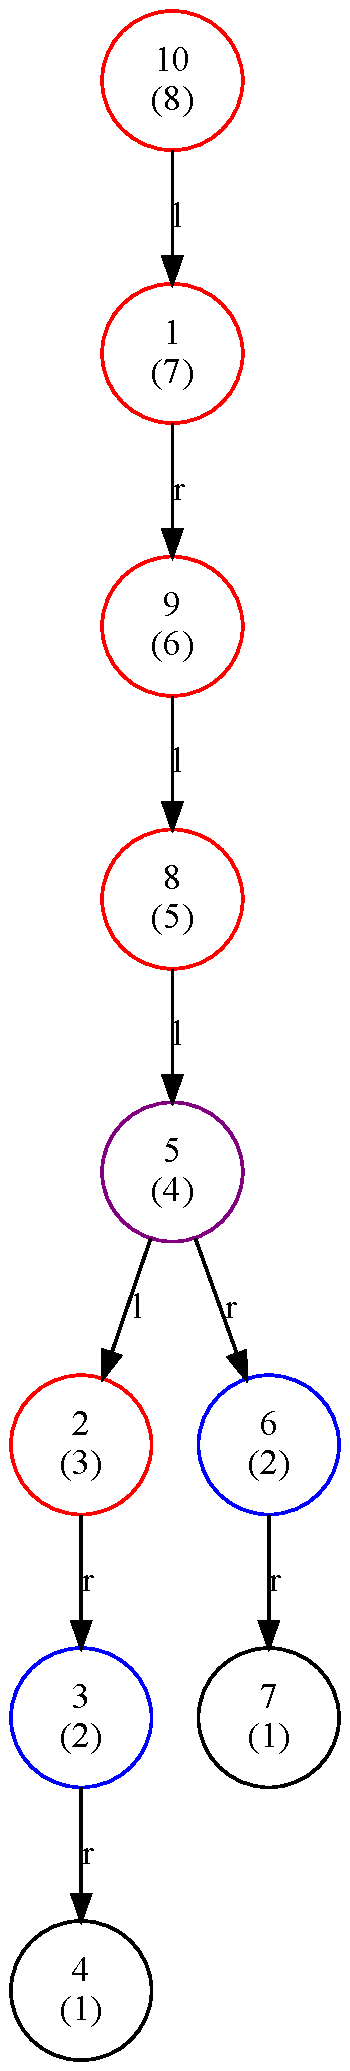
\includegraphics[scale = 0.32]{img/gv/aufg2_6_Insert10}\label{fig:splay-insert10}}
    \qquad
    \subfloat[\centering FindTP 99]{
        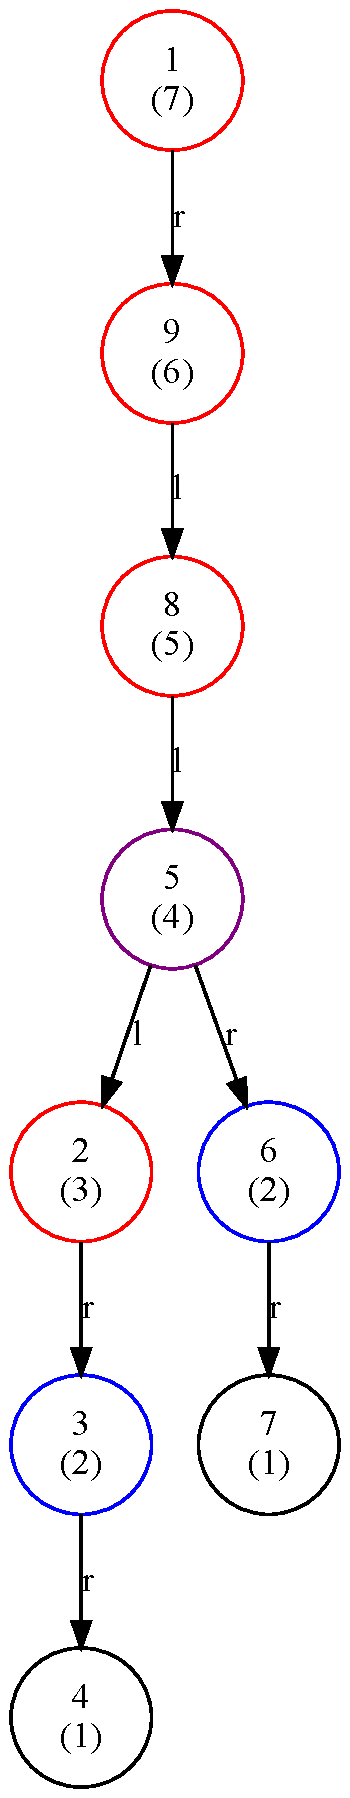
\includegraphics[scale = 0.32]{img/gv/aufg2_6_FindTP99}\label{fig:splay-findtp99}}
    \qquad
    \subfloat[\centering Delete 99]{
        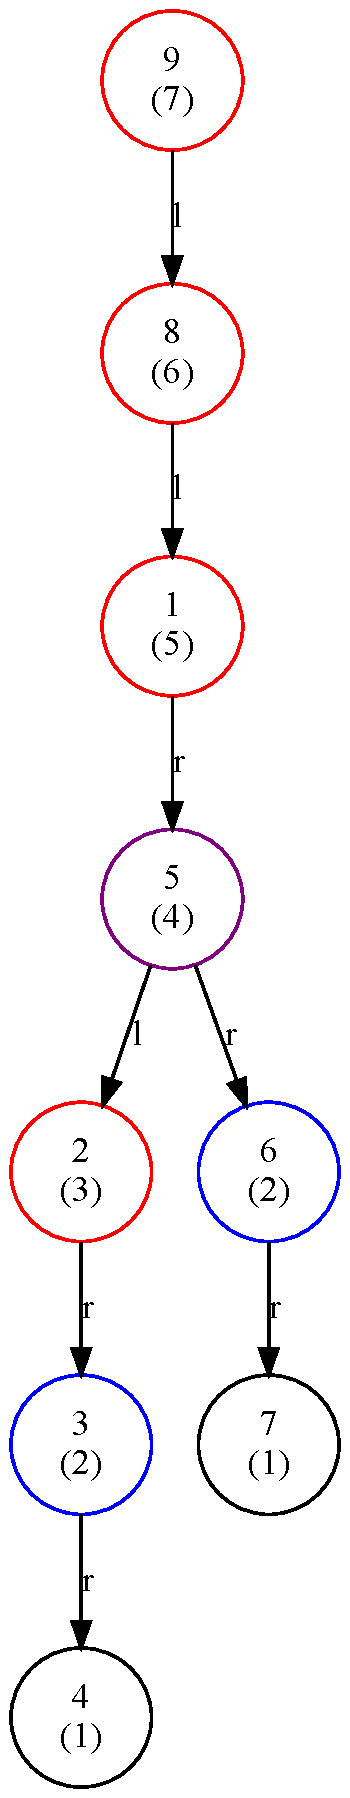
\includegraphics[scale = 0.32]{img/gv/aufg2_6_Delete99}\label{fig:splay-delete99}}
    \qquad
    \subfloat[\centering FindBT 99]{
        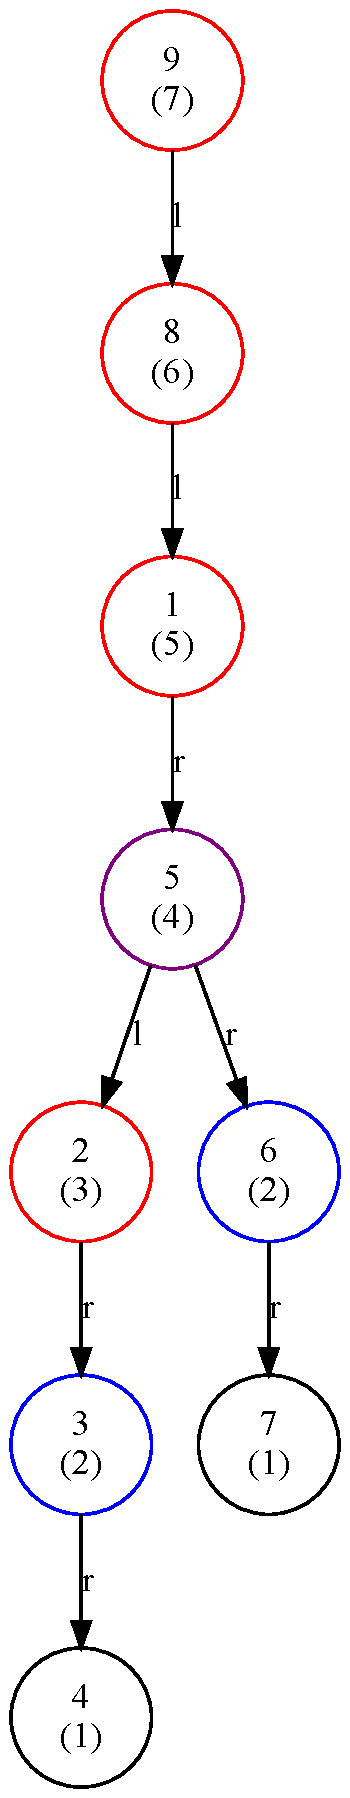
\includegraphics[scale = 0.32]{img/gv/aufg2_6_FindBT99}\label{fig:splay-findbt99}}
    \caption{Bilder der Splaying-Strategie - nicht vorhandene Elemente}\label{fig:splay2}
\end{figure}



\end{document}
